% FIRST OF ALL:
% If you are using X-based Emacs to read this file, please switch on
% Syntax Highlighting by typing:
%    ALT-X  font-lock-mode   (or META-X on X-Terminals)
%
% That should make these comments nice and red so they can be easily
% distinguished from the actual code. 
% =======================================================================

% This is a template for  Masters' Theses at WPI.
% It complies (more or less) to the standards given by the Library 
% (as of February 1999)
%
% Feel free to use this file, but I give no guarantee for its compliance
% to standards (meaning I won't pay for the paper if the library rejects it :))
%
%
% The lengths (textheight, width etc.) are fine-tuned for ps1, ps2, and ps3, 
% but seem to be somewhat dependent on the machine you are using to compile, 
% the date, time, moon phase, the weather, and other quantum effects.
% You may have to change \oddsidemargin a little, but it's about 98% correct.
%
% Also, the spacing is correct (doublespacing with footnotes correctly
% singlespaced). Curiously, the font size is not specified in the
% regulations. So feel free to change it, but the majority of theses
% that I have seen is written in 12 point font.
% 
% As for the inclusion of graphics, I recommend the methods specified
% in ``latexguide.ps'' off the CS-GSO Website. You can use other
% methods including copy and paste with a photocopier, but I think
% using the graphicx package is the easiest.
%
% Have fun and good luck with the thesis.
%
%
%  Andreas Koeller (koeller@wpi.edu)
%
%
%

% The preamble
%
%
% 12 point font, and your thesis is a ``report'' to LaTeX
\documentclass[12pt]{report}

% this enables correct linespacing and graphics inclusion via 
%``\includegraphics''
\usepackage{setspace}
\usepackage{graphicx}
\usepackage[tight, footnotesize]{subfigure}
\usepackage{algorithm}
\usepackage{algpseudocode}
\usepackage{multirow}
\usepackage{multicol}
\usepackage{amsmath}


% leave 1.5in margin to the left and 1in margin to the other
% sides. Don't print page number in the margin (but rather above it)
\setlength{\textheight}{8.63in}
\setlength{\textwidth}{5.9in}
\setlength{\topmargin}{-0.2in}
\setlength{\oddsidemargin}{0.3in}
\setlength{\evensidemargin}{0.3in}
\setlength{\headsep}{0.0in}

% Start to write
\begin{document}

% First things first: The Titlepage
% This is the recommended format by the library
%


% Define \brk as a command for leaving a little vertical space. Makes
% the titlepage easier to read - normally, this is NOT GOOD LATEX
% STYLE!!!
%
\newcommand{\brk}{\vspace*{0.18in}}

% No page number on the title page
\thispagestyle{empty}

% Center the whole title page
\begin{center}

\brk

% Large font and bold face for the headline. Try to keep it at one or
% two lines. Headlines over two lines will mess up the spacing, and you have to
% manually finetune it. Note that the line break in the SOURCE CODE
% does not affect the line breaking in the output file. If you want
% hardcoded line breaks, you have to mark them with a double backslash (\\)

   {\large 
	\textbf{
	Sensor Behavior Modeling and Algorithm Design for Intelligent Presence Detection in Nursery Rooms using iBeacon
	}
   }


\brk
by

\brk
% insert your name here. 
Zhouchi Li


% All this is constant:
\brk\brk
A Thesis

\brk
Submitted to the Faculty

\brk
of the 

\brk
WORCESTER POLYTECHNIC INSTITUTE
	
\brk
In partial fulfillment of the requirements for the

\brk
Degree of Master of Science

\brk
in

\brk
Electrical and Computer Engineering

\brk
by

% This is how LaTeX draws lines :) It's where your signature goes.
\brk\brk
\rule{3in}{1.2pt}

% Adjust this to your preferred month and year
\brk
April 2016

\end{center}

	
\vfill
APPROVED:

\vspace{0.5in}
\rule{3in}{0.8pt}

% Change this to your favorite CS professor.
Professor Kaveh Pahlavan, Major Thesis Advisor

\vspace{0.5in}
\rule{3in}{0.8pt}

% This is also constant :)
Professor Yehia Massoud, Head of Department	


% end of titlepage
\newpage

% This is the command for doublespacing when you use the setspace
% package
% Please do NOT use \baselinestretch, this will mess up everything,
% cause earthquakes, tornados and lots of questions for me...
% If you need a singlespaced paragraph (BAD STYLE!!!), use
% \singlespacing or \onehalfspacing and enclose it together with the
% paragraph in braces {\singlespacing This is my text... blah blah blah}
%
\doublespacing

% Now you can start to be creative.
% First, you need an abstract.
% Fortunately, LaTeX has thought of that, so it's very easy:
%
\begin{abstract}
This thesis is a part of a research project performed by two MS students Yang Yang and the author. 
The overall objective of the project is the design, implementation, and performance evaluation of algorithms for newborn localization and tracking in hospitals using Apple iBeacon technology.  In the research project, I lead the path-loss modeling of iBeacon, design of algorithms for in-room presence detection system, and analysis of the accelerometer sensor. My partner, Yang Yang, leads the performance evaluation of the localization system using Cramer Rao Lower Bound (CRLB). This manuscript describes the project with a focus on my contributions in modeling the behavior of sensors and presence detection algorithms. 

Today, RFID detection is the most popular indoor detection technique. It provides high precision detection rate to distinguish the number of people in certain rooms of a building. However, special scanners and manual operations are required. This increases the cost and operation complexity. With the recent introduction of iBeacon by Apple, possibility of more efficient in-room presence detection has emerged for specific applications. An example of these applicatons is recording the number of visitors and newborns in a nursery room inside a hospital. The iBeacon uses Bluetooth Low Energy (BLE) technology for proximity broadcasting. Additionally, iBeacon carries a motion detection sensor, which can be utilized for counting the number of people and newborns entering and leaving a room.

In this thesis we introduce a novel intelligent in-room presence detection system using iBeacon for the newborns in hospitals to determine the number of visitors and newborns' location in the nursery room. We first develop a software application on iPhone to receive and extract the necessary data from iBeacon for further analysis. We build the path-loss model for the iBeacon based on the received signal strength (RSS) of the iBeacon, which is used for performance evaluation using CRLB in Yang Yang’s project. We also utilize the accelerometer in the smart phones to improve the performance of our detection system.
\end{abstract}

% From here on, we need Roman page numbers according to the library
% regulations. So let's assign those.

\pagenumbering{roman} % or {Roman} if you like them capitalized

% The next thing is the Preface (``Acknowledgements'').
% No standard environment for that, so we'll format it by hand.
%
\begin{center}
	\textbf{Acknowledgements}
\end{center}
This thesis is a summary of my research work during the one-and-a-half-years in pursuit of my Master of Science Degree in Electrical \& Computer Engineering in Worcester Polytechnic Institute.

Firstly, I would like to offer my sincerest gratitude to my research advisor, Professor Kaveh Pahlavan, for leading me into the research field, for sharing his idea and life experience, and for providing working opportunity in his conference. Professor Pahlavan is a kindly mentor and a wise man. It is my greatest honor to have him as my advisor. 

I am really grateful that I can have Professor Emmanuel O. Agu and Professor Xinming Huang as my thesis committee members. Thank you for the careful review and valuable comments to this thesis. 

I would like to thank my partner Yang Yang. We work together throughout the master period. Most of the contributions in our research comes from cooperation and collaberation. I really enjoy the time studying and working with Yang.

I also want to thank all the peers in the center for wireless information network studies (CWINS), including Yishuang Geng, Julang Ying, Yuzhang Zang, Bader A. Alkandari, and Professor Dan Liu. Thank these people so much for offering me a nice atmosphere in the lab like a big family. I would like to give my especially thank to Yishuang. Over the one year and a half, he gives me plenty of help in both study and life. I cannot give a certain number that how many times he helped me until midnight. 

I would like to delicate my thesis to my beloved parents, who offer me totally understanding, support and infinity love. Also to my grandparents, who are always proud of me.

% P.S. You don't have to add me to the acknowledgements for providing 
% this file :)

\clearpage


% Now comes the Table of Contents, really easy in LaTeX. you never
% have to worried about it. (Think of all the hours you would
% have wasted in Word getting this thing updated without crashing
% the system) :).

\tableofcontents

% THAT'S IT. REALLY. Everything else is automatic. No formatting, no headline.
% All predefined.

% Now - just as easy - the List of Figures.
% This will catch all objects enclosed in \begin{figure}\end{figure}
% statements.
\listoffigures

% There is also a list of tables, if you have any.
% This will catch all objects enclosed in \begin{table}\end{table}
% statements.
\listoftables


% And we need a clear separation between preface and text, otherwise
% the numbering gets confused.

\clearpage

% And now - tataa - the text.
% This is the place to become really creative.

% From here on, we need arabic numbering again and we need to start
% from 1.

\pagenumbering{arabic}
\setcounter{page}{1}

% 
% Since this is a ``report'', the topmost level of hierarchy is
% ``Chapter'', not section as you may be used to. Chapters are
% enumerated starting from 1, so Sections are 1.1, Subsections are
% 1.1.1, subsubsections don't get numbers. (You can change that, if
% you want them to be called 1.1.1.1)
%
\chapter{Introduction}
iBeacon is a class of Bluetooth Low Energy (BLE) devices that broadcast unique information to the nearby receivable devices. The unique information packet includes Universally Unique Identifier (UUID), major, and minor. iBeacon constantly and periodically sents out beacon signals and all of them can be defined by the user. When these iBeacons are detected, the receivers can estimate the proximity as a reaction according to the Received Signal Strength Indication (RSSI) of the iBeacon. In brief, iBeacon is like the beacon in the ocean. It sends Bluetooth Low Energy signal instead of light to the receivers. 

Compared with traditional Bluetooth technology, iBeacon with BLE signal is intended to have similar coverage area yet less power consumption. With this advantage, iBeacon can be used for years without changing battery. Due to the broadcasting nature, the devices using BLE signal do not need to pair with each other when they communicate. Most of the smart phones, such as iPhone, Android and Blackberry, are compatible with BLE technology which indicates that they can perform collaborative operations with iBeacon~\cite{ens}. It is also expected to apply BLE on Windows Phones soon. That means we do not need to install special BLE receivers for iBeacon since almost everyone has a smart phone.

\section{Background and Motivation}
iBeacon has many location-based applications. It can be used to develop indoor positioning systems~\cite{mar}~\cite{gen15a}. It can be used to build an indoor proximity estimation system to detect the number of moving objects in the surrounding area, and even gather the patterns of their movement~\cite{cor}. Moreover, iBeacons can be also used as a trigger to launching APPs on remote devices~\cite{bas}. The interest of industry for iBeacon is increasing as well. Not only Apple but enterprises such as Qualcomm, PayPal, and SKT carry forward related businesses by partnering with a variety of companies and organizations~\cite{kim}.

There are some differences between iBeacon and other traditional wireless communication technologies. First, the signal that iBeacon transmits is a one-way broadcast, which means only the receiving devices can get information from iBeacon, but not the other way around. Second, users have to install an application on their smartphones or other receiving devices before they use them to receive BLE signal. This will help users to protect their privacy because the one-way communication mechanism guarantees that their position information is difficult to intercept and is only locally stored on the installed APP.

The iBeacon implementation systems usually consist of several iBeacons, receivers with preloaded software, and servers. The iBeacons send signal to the proximate area. The receivers search the iBeacons signal and run certain applications according to the received signal. Note that the signal just provide an identifier and trigger the applications on receiving devices. It is the applications' job to do the rest things such as sending notifications and navigation.

The basic function of the iBeacon is providing proximity information based on the RSSI. Applications can get the approximate distance or the range to a certain iBeacon since the RSSI declines with the increment of distance. With the distance or ranging information, a lot of things can happen. The iBeacon on the door can notify the entry/exit of the room. The iBeacon in the store can push introduction and discount of goods to the nearby customers. The iBeacon under the table can let customers order food by themselves. 

The packet that iBeacon broadcasts is editable. By defining the packet of every iBeacon we can distinguish the iBeacon we scaned, which makes the multi-iBeacon systems possible. If we can look up several iBeacons at the same time, more complex applications like indoor localization is realizable. Users can also change the advertising interval and transmit power to a proper value. Higher advertising frequency and transmit power will increase both accuracy and power consumption, so users have to make a trade-off between them.

The efficient power consumption is a main difference between the BLE and classic bluetooth. Several chipsets makers have already launched optimized iBeacon chips. The power consumption of iBeacon mostly depends on the advertising interval and transmit power. The iBeacon we used can provide four months of battery life under the 100 ms advertising interval, which is the minimum interval value of the iBeacon. The battery life can be extended to more than two years if we set the advertising interval to 1000 ms.

The power consumption of the smartphones should also be considered. The applications running on the smartphones will decrease the battery life. However, the loss can be controlled in a reasonable range since the applications can run in the background for most of the time. Even running in the background, the applications are able to scan iBeacons nearby. 

With the advancement of localization technology, outdoor localization is quite mature and has been implemented in our daily life such as the vehicle navigation and physical distribution. Nowadays there are a huge amount of indoor smartphone applications which have an intense need to the position information of the users. With the help of the information, plenty of position-based applications are achievable. However, the traditional outdoor localization technologies cannot solve the problem successfully. 

\section{Contribution}
The thesis consists of two major sections and the major contribution of this thesis has been listed as follows:

\begin{itemize}
\item Development of the intelligent in-room presence detection system by using iBeacon \\
\hspace{10mm} (1) Developing different algorithms \\
\hspace{10mm} (2) Analysing the performance of the algorithms
\end{itemize}

\begin{itemize}
\item Development of the in-room localization by using iBeacon \\
\hspace{10mm} (1) Building the pathloss model \\
\hspace{10mm} (2) Validating the pathloss model \\
\hspace{10mm} (3) Analysing the effect of 3D deployment patterns 
\end{itemize}

In the first major section we collected data for line-of-sight (LOS) situation in in-room environment, and then recognize in-room presence according to path-loss variations. Data in other situations and environments such as obstructed-line-of-sight (OLOS) and outdoor scenario has been also considered to guarantee the in-room presence detection accuracy. Based on the empirical measurement results, we deeply investigate the system performance in terms of error detection possibility. This system is specifically promising for some particular purposes such as graduate seminar check-in, security system, in-and-out counting.

In the second major section we developed a new application to obtain the necessary data from iBeacon and then derive the real path-loss model for line-of-sight (LOS) situation in in-room environment on account of received signal strength indication (RSSI) analysis. Besides, we apply the iBeacon model used in Estimote iBeacons~\cite{estlink} and compare the performance of those two models. Simulation results of Cramér-Rao Lower Bound (CRLB) estimation of location error model are also calculated in this paper considering 2D and 3D scenarios respectively. After the feasibility analysis we conclude our work with a discussion on the feasibility of using iBeacon for locating and tracking rather than RFID, especially in hospitals~\cite{che}.

\section{Thesis Outline}
This thesis is organized as follow: Chapter 1 provided a brief introduction to the iBeacon technology. Chapter 2 introduced the background of the iBeacon based system by presenting hardware components, software development environments, and system integration. Chapter 3 discussed the intelligent in-room presence detection system and associate detection algorithms. Chapter 4 proposed the real path-loss model of iBeacon and validated and evaluated the path-loss model based on CRLB. Last but not the least, Chapter 5 presented the conclusion of this thesis and discussion of the future work. 

%%%%%%%%%%%%%%%%%%%%%%%%%%%%%%%%%%%%%%%%%%%%%%%%%%%%%%%%%%%%%%%%%%%%%%%%%%%%%%%%%%%%%%
%%%%%%%%%%%%%%%%%%%%%%%%%%%%%%%%%%%%%%%%%%%%%%%%%%%%%%%%%%%%%%%%%%%%%%%%%%%%%%%%%%%%%%
%%%%%%%%%%%%%%%%%%%%%%%%%%%%%%%%%%%%%%%%%%%%%%%%%%%%%%%%%%%%%%%%%%%%%%%%%%%%%%%%%%%%%%
%										Chapter 2
%%%%%%%%%%%%%%%%%%%%%%%%%%%%%%%%%%%%%%%%%%%%%%%%%%%%%%%%%%%%%%%%%%%%%%%%%%%%%%%%%%%%%%
%%%%%%%%%%%%%%%%%%%%%%%%%%%%%%%%%%%%%%%%%%%%%%%%%%%%%%%%%%%%%%%%%%%%%%%%%%%%%%%%%%%%%%
%%%%%%%%%%%%%%%%%%%%%%%%%%%%%%%%%%%%%%%%%%%%%%%%%%%%%%%%%%%%%%%%%%%%%%%%%%%%%%%%%%%%%%

\chapter{Background and Application Develpment Environment}
In order to utilize iBeacon for either in-room presence detection or in-room localization, it is necessary to build a system, which can measure the physical, environmental information and at the same time perform computational tasks. As for sensing or measuring the physical signal, the hardware components of the system in this thesis include:

\begin{itemize}
\item Several pre-deployed iBeacons. The iBeacons is periodically emmiting BLE signal, they work as the signal sources of the system.
\item A smart phone. The smart phone is carried by the users, it works as the receiver/reader of the BLE signal and may perform limited computation.
\item A laptop. The laptop works as a centroid server. One the one hand, it performs most of the comptational tasks, and on the other hand, it can work as a coordinator for multiple users.
\end{itemize}

As for data processing, data forwarding and algorithm implementation, there are two separate parts of software in the system including:

\begin{itemize}
\item An iOS application running on the smart phone. This application is in charge of data collection. After collecting raw data, it will forward useful data to the server.
\item An command line programm running on the laptop(server). The server program is where we implement the algorithms and properly announce and maintain a database of algorithm outputs.  
\end{itemize}

This chapter has been divided into three sections. In section 2.1, we provide detailed introduction of the selected iBeacon. In section 2.2, we anaylze the disadvantage of existing, commercialized iOS applications and propose our self-designed iOS APP. Finaly in section 2.3, we offer an integrated view of the entire system with a focus on how is the data is collected and how the data exchanges between iOS client and the server. With this chapter serving as a background, it is easier for the readers to understand the following of this thesis.


\section{Hardware Devices}
In this project we use the iBeacon producted by Estimote. We use iBeacon of 2 different generations. The first generation is shown as Fig~\ref{fig: 3.2}.

\begin{figure}[htb]
	\begin{center}
		\begin{tabular}{c}
			\scalebox{0.5}{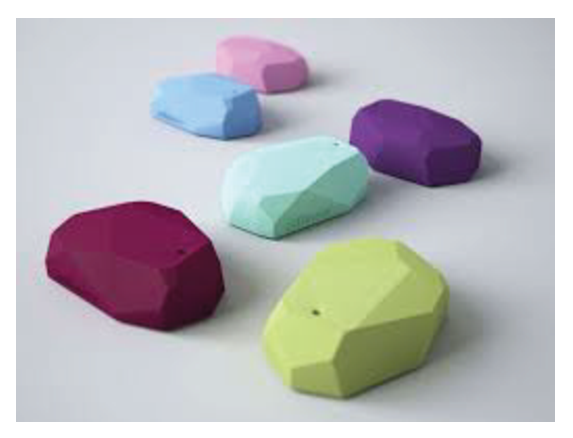
\includegraphics[]{pictures/3_2.eps}}
		\end{tabular}
	\end{center}
	\caption{First Generation iBeacon of Estimote.}
	\label{fig: 3.2}
\end{figure}

We did most of the project by using the first generation iBeacon. It is a 3cm $\times$ 2cm $\times$ 1cm plastic lump with BLE transmitter, motion detection sensor, and temperature sensor in it. The BLE transmitter and motion detection sensor are the modules we use. BLE transmitter provides us RSSI value of the iBeacon. With that data we can get the distance range between the iBeacon and receiver. Combined with the path-loss model we can even get the distance. When the iBeacon is moved, the motion detection sensor will send a special signal which is very useful. Then we know when the door is opened and closed. 

The parameters of iBeacon are editable. Users can define the parameters by themselves on the application. The parameters include Universal Unique Identifier, advertising interval, transmit power, and so on. The range of the advertising interval is from 100ms to 2000ms. The higher the transmit power and advertising frequency we set, the shorter the battery life will be. 

\begin{figure}[htb]
	\begin{center}
		\begin{tabular}{c}
			\scalebox{0.7}{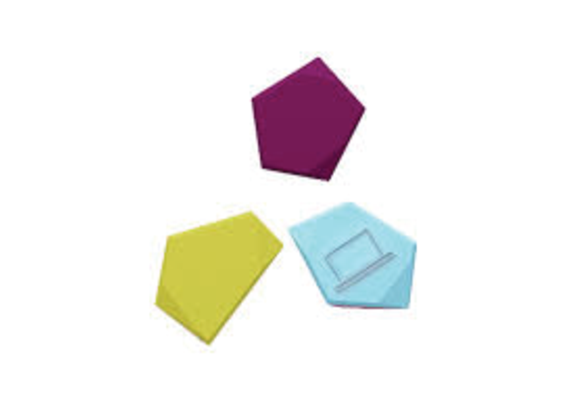
\includegraphics[]{pictures/3_3.eps}}
		\end{tabular}
	\end{center}
	\caption{Second Generation iBeacon of Estimote.}
	\label{fig: 3.3}
\end{figure}

We also bought the second generation iBeacon, which is shown as Fig~\ref{fig: 3.3}. The second generation iBeacon is smaller than the first generation. It is only several millimeters high so it looks flat. Since it has less space, the battery life is shorter than the first generation. However, there is an accelerometer in it. Now it can provide not only the motion status of iBeacon but also the acceleration on three dimensions. Because of the tiny volume, the second generation iBeacon can be put on moving objects easily and provide the acceleration and velocity information of the objects.

The hardware we use in this project is the iBeacon from Estimote company. The iBeacon provides 3 kinds of important data. They are iBeacon id, RSSI, motion status. 

The iBeacon id is 20 bytes long and composed of 3 parts: UUID, major, and minor. All of them can be defined by users. 

\begin{itemize}
\item 3 sections of iBeacon id:

\labelitemiv UUID (16 bytes)

\labelitemiv major (2 bytes)

\labelitemiv minor (2 bytes)

\end{itemize}

The iBeacon id can be regarded as a three-dimensional string. Imaging there is one iBeacon in each room of the campus. The UUID illustrates the building number. The major is used to show the floor number. The minor number refers to the room number. Now every iBeacon in the room has a unique iBeacon id. If we receive the signal of a certain iBeacon, we can find out which iBeacon it is and which room it is in.

In this project, iBeacon id is used to distinguish which iBeacon we are communicate with. In some cases we have to detect and record RSSI of 2 iBeacons. In real scenario the number of iBeacon we have to monitor at the same time will be even more. Thus, it is necessary to distribute a unique id to every iBeacon.

The RSSI of iBeacon is the most important information that iBeacon provide. As we know, the closer the distance between the iBeacon and receiver is, the higher the RSSI value we will receive. In this project, RSSI is the parameter to compare the relative distance between several iBeacons and receiver, and the movement scenario of the user. The RSSI is received by iPhone in our project, and then sent to a Macbook which is used as server. The server will store the data and let us do post processing.

The motion detection sensor in the iBeacon will send a special signal when the iBeacon is moved. This means we will be noticed once the object attached by iBeacon has movement. If we put the iBeacon on the door, the status of the door will be monitored in real time.

\section{Software Application}
The term iBeacon and Beacon are often used interchangeably. iBeacon is the name for Apple’s technology standard, which allows Mobile Apps (running on both iOS and Android devices) to listen for signals from beacons in the physical world and react accordingly. In essence, iBeacon technology allows Mobile Apps to understand their position on a micro-local scale, and deliver hyper-contextual content to users based on location. The underlying communication technology is Bluetooth Low Energy.

Bluetooth Low Energy is a wireless personal area network technology used for transmitting data over short distances. As the name implies, it’s designed for low energy consumption and cost, while maintaining a communication range similar to that of its predecessor, Classic Bluetooth.

In a word, BLE is different from Regular Bluetooth in 3 main aspects:

\begin{itemize}
\item Power Consumption: Bluetooth LE, as the name hints, has low energy requirements. It can last up to 3 years on a single coin cell battery.
\item Lower Cost: BLE is 60-80\% cheaper than traditional Bluetooth.
\item Application: BLE is ideal for simple applications requiring small periodic transfers of data. Classic Bluetooth is preferred for more complex applications requiring consistent communication and more data throughput.
\end{itemize}

With an iBeacon network, any brand, retailer, app, or platform will be able to understand exactly where a customer is in the brick and mortar environment. This provides an opportunity to send customers highly contextual, hyper-local, meaningful messages and advertisements on their smartphones.

The typical scenario looks like this. A consumer carrying a smartphone walks into a store. Apps installed on a consumer’s smartphone listen for iBeacons. When an app hears an iBeacon, it communicates the relevant data (UUID, Major, Minor, Tx) to its server, which then triggers an action. This could be something as simple as a push message [“Welcome to Target! Check out Doritos on Aisle 3!”], and could include other things like targeted advertisements, special offers, and helpful reminders [“You’re out of Milk!”]. Other potential applications include mobile payments and shopper analytics and implementation outside of retail, at airports, concert venues, theme parks, and more. The potential is limitless.

This technology should bring about a paradigm shift in the way brands communicate with consumers. iBeacon provides a digital extension into the physical world. We’re excited to see where iBeacon technology goes in the next few years. Depending on how iBeacon evolves and is adopted it could form an important part of Apple's ecommerce and mobile payments effort. For example, the combination of iBeacon and Passbook could allow you to get sent a coupon while in a store and buy something without ever seeing a member of staff. Equally, shoppers may find the whole thing slightly unnerving and ignore it altogether. This is why iBeacon is a Big Deal.

\subsection{Estimote iBeacon APP}
In our project, we use Estimote iBeacons as our main devices, meanwhile, Estimote company provides us an existing application in iBeacon. Here we provide some figures about this application.

When an eligible mobile app enters the signal's region, corresponding actions can be triggered. Estimote SDK and Cloud tie everything together by granting apps access to additional features, including security layer, fleet management, and indoor location. Phones or other smart devices can pick up the beacon’s signal and estimate the distance by measuring received signal strength (RSSI). The closer you are to the beacon, the stronger the signal. Remember that the beacon is not broadcasting continuously—it’s blinking instead. The more frequent the blinks, the more reliable the signal detection. And because Bluetooth Smart doesn’t require pairing, a phone can listen to many beacons at the same time. This unlocks more opportunities: for example indoor location.

\begin{figure}[!t]
	\centering
	\subfigure[]{
		\begin{minipage}[htb]{0.35\textwidth}
			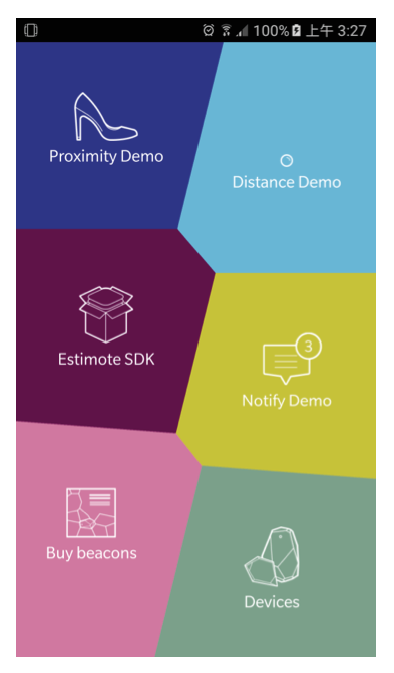
\includegraphics[width = 1\textwidth]{pictures/3_4a.eps}
		\end{minipage}
	}
	\subfigure[]{
		\begin{minipage}[htb]{0.35\textwidth}
			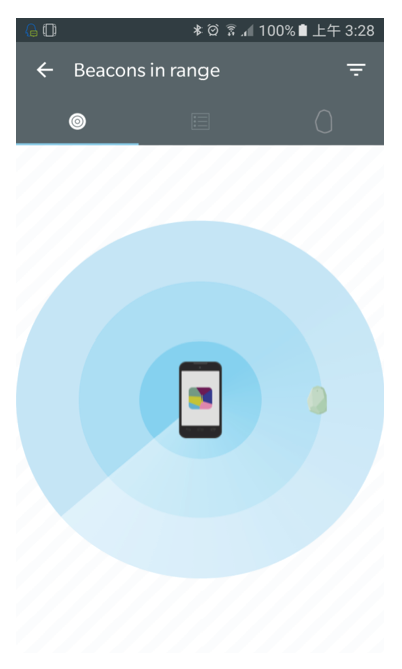
\includegraphics[width = \textwidth]{pictures/3_4b.eps}
		\end{minipage}
	}
	\\
	\subfigure[]{
		\begin{minipage}[htb]{0.35\textwidth}
			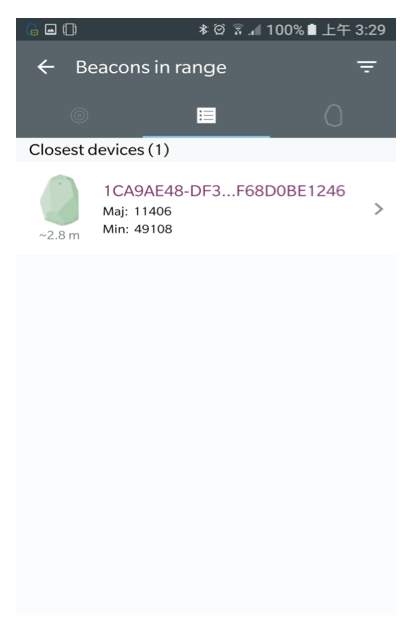
\includegraphics[width = \textwidth]{pictures/3_4c.eps}
		\end{minipage}
	}
	\subfigure[]{
		\begin{minipage}[htb]{0.35\textwidth}
			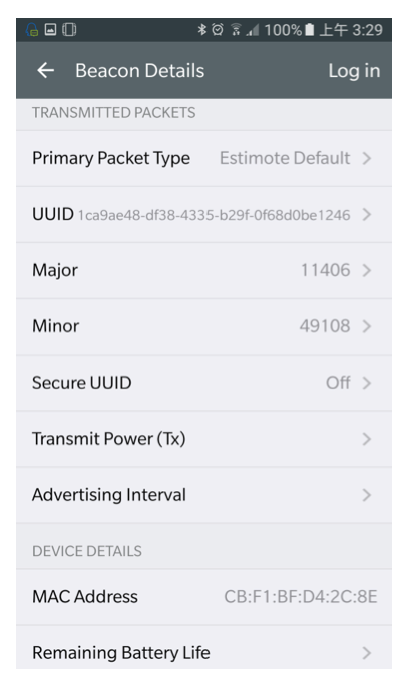
\includegraphics[width = \textwidth]{pictures/3_4d.eps}
		\end{minipage}
	}
	\caption{Screenshots of Estimote iBeacon Application.}
	\label{fig: 3.4}
\end{figure}

From Fig~\ref{fig: 3.4} we can see that based on this application, we can not only find out the approximate distance between iBeacon and iPhone, but also obtain the necessary data such as RSSI, major, minor, UUID and even MAC address. This is quite useful for a fresh man to understand how iBeacon works and how to use iBeacon.

\subsection{Self-designed iBeacon APP}
The iBeacons produced by estimote company can provide us much information we need such as RSS, broadcasting interval, minor and major values and even motion sensor. However, the existing app from extimote company do not allow us to collect data directly from iphone which means large samples are impossible and we can only collect data by hand. 

Even though the application provided by Estimote company can satisfy many requirements in iBeacon, there is an unavoidable problem existing in this application: we cannot extract any data from this application, which means the RSS data we need can only be recorded by hand that is absolutely inconvenient and impossible for large data. To solve this problem, we decide to develop our own app.

\begin{figure}[htb]
	\begin{center}
		\begin{tabular}{c}
			\scalebox{0.9}{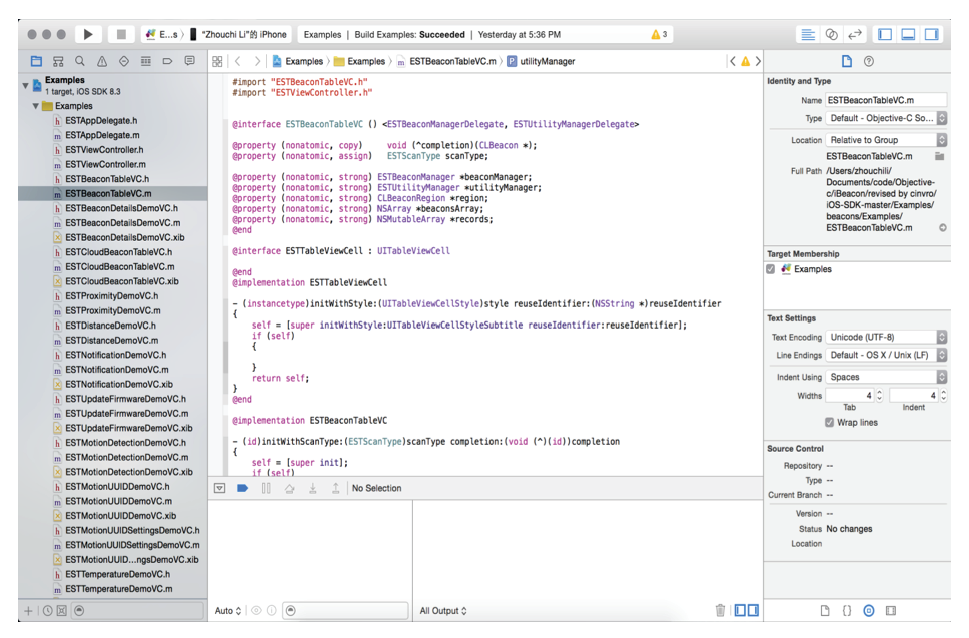
\includegraphics[]{pictures/3_5.eps}}
		\end{tabular}
	\end{center}
	\caption{Objective-C Code Example.}
	\label{fig: 3.5}
\end{figure}

Estimote Indoor Location SDK allows real-time beacon-based mapping and indoor location. We know that building the next generation of context-aware mobile apps requires more than just iBeacon™ hardware. That's why we've built smarter software that abstracts away the difficulty of understanding proximity and position within a given space. Estimote Indoor Location is a sophisticated software solution that makes it incredibly easy and quick to map any location. Once done, you can use our SDK to visualize your approximate position within that space in real-time, in your own app. Indoor Location creates a rich canvas upon which to build powerful new mobile experiences, from in-venue analytics and proximity marketing to frictionless payments and personalized shopping. Estimote Indoor Location works exclusively with Estimote Beacons.

When it comes to our project, we use Objective-C to develop our app to get the RSS of the beacons. The iPhone 5s acts as the receiver in our research and it is connected to a Mac book computer by a cable. When it gets the packets from iBeacons which are in the detection range, it will display the current values of RSS both on the iPhone screen and Mac book computer. The data we collected in different situation can be used to do the channel modeling. Fig~\ref{fig: 3.5} is an example coding in Xcode using Objective-C.

\begin{figure}[htb]
	\begin{center}
		\begin{tabular}{c}
			\scalebox{0.9}{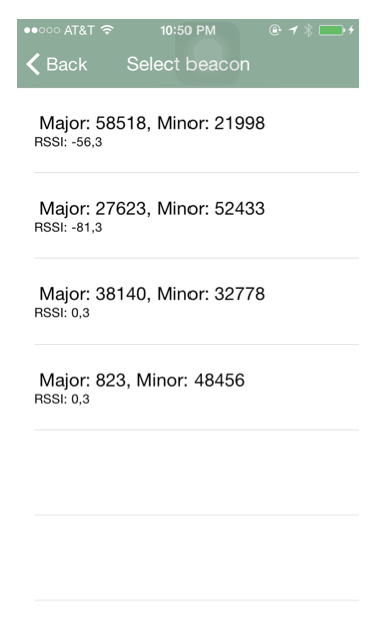
\includegraphics[]{pictures/3_6.eps}}
		\end{tabular}
	\end{center}
	\caption{Screenshots of Our Own iBeacon Application.}
	\label{fig: 3.6}
\end{figure}

\begin{figure}[htb]
	\begin{center}
		\begin{tabular}{c}
			\scalebox{0.9}{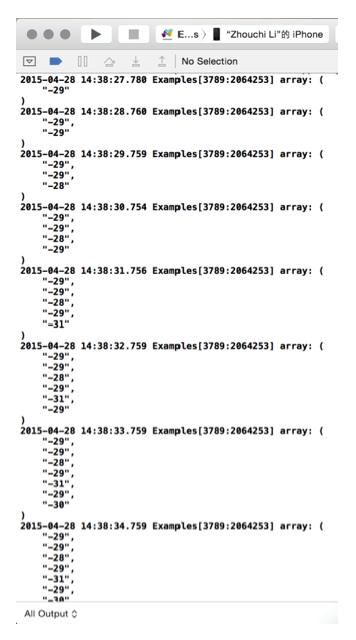
\includegraphics[]{pictures/3_7.eps}}
		\end{tabular}
	\end{center}
	\caption{Data Extracted from Our Own iBeacon Application.}
	\label{fig: 3.7}
\end{figure}

\begin{figure}[htb]
	\begin{center}
		\begin{tabular}{c}
			\scalebox{0.9}{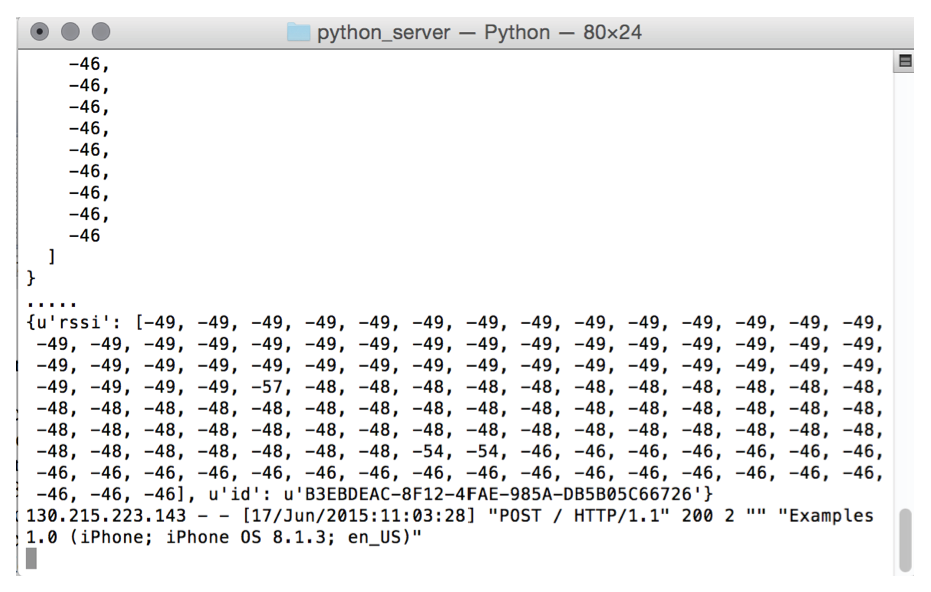
\includegraphics[]{pictures/3_8.eps}}
		\end{tabular}
	\end{center}
	\caption{Our Server for the System.}
	\label{fig: 3.8}
\end{figure}

\section{Integrated Experimental System}
Fig~\ref{fig: 3.6} shows the app we have developed based on the API provided by Estimote Company. It can show the list of the beacons detected by our device and take down the RSS signal, major, minor, sequence number of the data and whatever information of beacons we want. As shown in Fig~\ref{fig: 3.7} our need of extracting the RSS data can be satisfied by the app.

Fig~\ref{fig: 3.8} shows the server we built on my computer by using Python. After the smart phone application captures the BLE signal, the raw data will be forwarded to this server in real-time. The server opens a TCP socket over the WiFi network connection and seamlessly collect the raw data. The RSSI for each specific iBeacon id has been extracted from the raw data and forms process data in tuples. each tuple contains several field including time stamp, iBeacon id and the RSSI. The processed data can be then used as the direct input of either in-room presence detection algorithm or in-room localization algorithm. Also, we can do numerical analysis in Matlab in the design/development phase of our agorithms.



%%%%%%%%%%%%%%%%%%%%%%%%%%%%%%%%%%%%%%%%%%%%%%%%%%%%%%%%%%%%%%%%%%%%%%%%%%%%%%%%%%%%%%
%%%%%%%%%%%%%%%%%%%%%%%%%%%%%%%%%%%%%%%%%%%%%%%%%%%%%%%%%%%%%%%%%%%%%%%%%%%%%%%%%%%%%%
%%%%%%%%%%%%%%%%%%%%%%%%%%%%%%%%%%%%%%%%%%%%%%%%%%%%%%%%%%%%%%%%%%%%%%%%%%%%%%%%%%%%%%
%										Chapter 3
%%%%%%%%%%%%%%%%%%%%%%%%%%%%%%%%%%%%%%%%%%%%%%%%%%%%%%%%%%%%%%%%%%%%%%%%%%%%%%%%%%%%%%
%%%%%%%%%%%%%%%%%%%%%%%%%%%%%%%%%%%%%%%%%%%%%%%%%%%%%%%%%%%%%%%%%%%%%%%%%%%%%%%%%%%%%%
%%%%%%%%%%%%%%%%%%%%%%%%%%%%%%%%%%%%%%%%%%%%%%%%%%%%%%%%%%%%%%%%%%%%%%%%%%%%%%%%%%%%%%

\iffalse

\section{RF-based Localization}


\section{Inertia-based Localization}
The paper [3-D Localization of Human Based on an Inertial Capture System] introduces a method to track the spatial location and movement of a human using wearable inertia sensors without additional external global positioning devices. Starting from the lower limb kinematics of a human, the method uses multiple wearable inertia sensors to determine the orientation of the body segments and lower limb joint motions. At the same time, based on human kinematics and locomotion phase detection, the spatial position and the trajectory of a reference point on the body can be determined. An experimental study has shown that the position error can be controlled within 1-2\% of the total distance in both indoor and outdoor environments. The system is capable of localization on irregular terrains (like uphill/downhill). From the localization results, the ground shape and the height information that can be recovered after localization experiments are conducted. A benchmark study on the accuracy of this method was carried out using the camera-based motion analysis system to study the validity of the system. The localization data that are obtained from the proposed method match well with those from the commercial system. Since the sensors can be worn on the human at any time and any place, this method has no restriction to indoor and outdoor applications.

\section{Camera-based Localization}
In the paper [MonoSLAM: Real-Time Single Camera SLAM], they present a real-time algorithm which can recover the 3D trajectory of a monocular camera, moving rapidly through a previously unknown scene. Their system, which they dub MonoSLAM, is the first successful application of the SLAM methodology from mobile robotics to the \"pure vision\" domain of a single uncontrolled camera, achieving real time but drift-free performance inaccessible to structure from motion approaches. The core of the approach is the online creation of a sparse but persistent map of natural landmarks within a probabilistic framework. Their key novel contributions include an active approach to mapping and measurement, the use of a general motion model for smooth camera movement, and solutions for monocular feature initialization and feature orientation estimation. Together, these add up to an extremely efficient and robust algorithm which runs at 30 Hz with standard PC and camera hardware. This work extends the range of robotic systems in which SLAM can be usefully applied, but also opens up new areas. They present applications of MonoSLAM to real-time 3D localization and mapping for a high-performance full-size humanoid robot and live augmented reality with a hand-held camera.

\fi

\iffalse

\chapter{Methodology for Application Development}
iBeacon is a class of Bluetooth Low Energy (BLE) devices that broadcast unique information to the nearby receivable devices. When these iBeacons are detected, the receivers can estimate the proximity as a reaction. Compared with traditional Bluetooth technology, iBeacon with BLE signal is intended to have similar coverage area yet less power consumption. Most of the smart phones, such as iPhone, Android and Blackberry, are compatible with BLE technology which indicates that they can perform collaborative operations with iBeacon. It is also expected to apply BLE on Windows Phones soon. 

iBeacon has many location-based applications. It can be used to develop indoor positioning systems [1][2]. It can be used to build an indoor proximity estimation system to detect the number of moving objects in a room, and even gather the patterns of their movement [3]. Moreover, iBeacons can be also used as launching APPs on remote devices [4]. The interest of industry for iBeacon is increasing as well. Not only Apple but enterprises such as Qualcomm, PayPal, and SKT carry forward related businesses by partnering with a variety of companies [5]. 

\begin{figure}[!t]
	\centering
	\subfigure[]{
		\begin{minipage}[htb]{0.5\textwidth}
			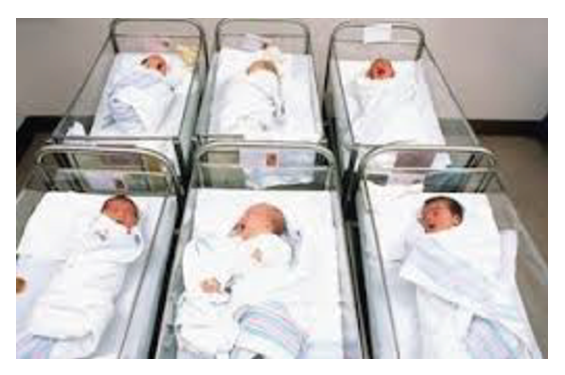
\includegraphics[width = 1\textwidth]{pictures/3_1a.eps}
		\end{minipage}
	}
	\\
	\subfigure[]{
		\begin{minipage}[htb]{0.5\textwidth}
			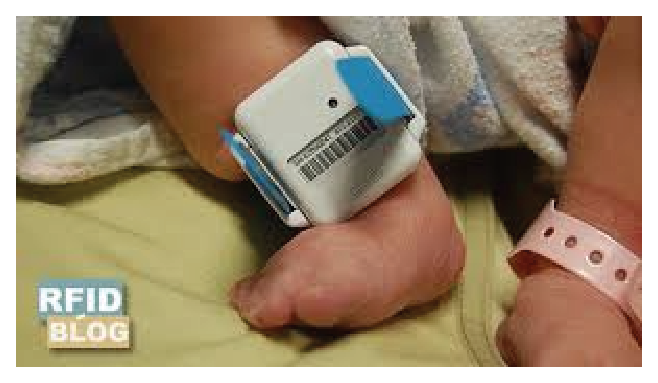
\includegraphics[width = \textwidth]{pictures/3_1b.eps}
		\end{minipage}
	}
	\caption{RFID Tag Used in Nursery Room.}
	\label{fig: 3.1}
\end{figure}

As mentioned above, iBeacon has a lot of advantages when it is compared with other in-room localization technologies. Thus, we want to use iBeacon to do nursery room children identification. As shown in Fig~\ref{fig: 3.1}, currently RFID technology is used to identify children in the nursery room of the hospitals. However, if we put iBeacons on each babies' leg and some certain places in the room, we can record visiting people in the nursery room and identify and track the newborns with sub-meter accuracies. In this project, we use iBeacon which allows identification and recording of visitors with the capability of broadcasting additional information about the users to the smart devices in the proximity.

The hardware basis of this work is the iBeacon transmitters from Estimote [6], cooperating with the most recent iPhone 5s, 6/6Plus and 6s/6sPlus. There are BLE transmitter and motion detection sensor in the iBeacon. When the iBeacon is moved, the motion sensor will send a special signal. It is very useful in our system because it can notice us when the door is opened and closed. Together with the hardware, Estimote company also provide us software application which can show us a lot of useful information such as iBeacon ID and RSSI. However, the Estimote application only display the RSSI but does not provide any way to port the sensor reading for further analysis. In order to get the data for post processing, we developed our own application using existing Estimote software development kits which provide RSSI and the motion information. With the help of our application, the iPhone can get the real-time RSSI data and send them to a Macbook. The Macbook is regarded as the server in the system. The server uses socket to communicate with the application on iPhone. After extracting the data to the Macbook, we can do further analysis.

By measuring the RSSI data on different distances to the iBeacon, we built the path-loss model for iBeacon. According to the RSSI at 1 and 5 meters measured by Estimote application, we also got the path-loss model used by Estimote. Compared the two path-loss models, our path-loss model has a better performance. 

Then we moved on to the system. We designed two algorithms for the system to distinguish 3 basic scenarios of human movement. The algorithms are verified by the RSSI data we extracted in CWINS lab. The detection rate for the two scenarios are almost 100\%. We got the conclusion that single iBeacon approach is adequate.


\fi

%%%%%%%%%%%%%%%%%%%%%%%%%%%%%%%%%%%%%%%%%%%%%%%%%%%%%%%%%%%%%%%%%%%%%%%%%%%%%%%%%%%%%%
%%%%%%%%%%%%%%%%%%%%%%%%%%%%%%%%%%%%%%%%%%%%%%%%%%%%%%%%%%%%%%%%%%%%%%%%%%%%%%%%%%%%%%
%%%%%%%%%%%%%%%%%%%%%%%%%%%%%%%%%%%%%%%%%%%%%%%%%%%%%%%%%%%%%%%%%%%%%%%%%%%%%%%%%%%%%%
%										Chapter 3
%%%%%%%%%%%%%%%%%%%%%%%%%%%%%%%%%%%%%%%%%%%%%%%%%%%%%%%%%%%%%%%%%%%%%%%%%%%%%%%%%%%%%%
%%%%%%%%%%%%%%%%%%%%%%%%%%%%%%%%%%%%%%%%%%%%%%%%%%%%%%%%%%%%%%%%%%%%%%%%%%%%%%%%%%%%%%
%%%%%%%%%%%%%%%%%%%%%%%%%%%%%%%%%%%%%%%%%%%%%%%%%%%%%%%%%%%%%%%%%%%%%%%%%%%%%%%%%%%%%%

\chapter{Design of Intelligent In-Room Presence Detection}

With the previous chapter serving as a background of our system, it is clear that we deploy iBeacons as a BLE signal sources, employ a smart phone to measure the signal profile as row data, and use the sever to process the signal profile. In this chapter, we start to present the design and implementation of the intelligent in-room presence detection approaches. 

To facilitate the description of our algorithms, we assume that the entrance door automatically shuts after an individual goes into or out of the room. We first and foremost focus on the system implementation with two iBeacons, one of them attached to the outside of door while another mirroring at the inside. Such implementation provides adequate understanding on the physical phenomenon. After that, we move on to single iBeacon implementation, for which our system still performs well enough, but works with less expenses and more convenience. The performace of both algorithms are provided as an evaluation metric and we discuss the the effect of smart phone location at the end of this chapter.

\section{Background}
Presence detection is a common application for smart phones, which may contribute to energy-efficient intelligent lighting control, smart heating and air-conditioning, home security system and etc. In public area, the in-room presence detection technologies can be also used to count the registration and check-in of an event. Existing literature introduces two major technical trends to implement in-room presence detection systems. At the beginning stage, the research community mounts various sensors to the room ceiling and tries to cover the room as much as possible. Sujin et. al~\cite{you}, proposed a digital camera and image processing based presence detection system using intensity average variation to detect moving objects; Neubiberg et. al~\cite{iva}, presents a 360o rotational camera based approach to enhance the camera coverage. Visible light sensing technique has been also employed in such systems and it has been even commercialized as products~\cite{premalink}. 

The above mentioned first technical trend suffers from certain disadvantages. First and foremost, the pre-deployment of the infrastructure is not unified. Take the thePremaTM in~\cite{premalink} as an example, only single sensor is required to cover a squared room but multiple sensors are necessary for an irregularly shaped room. As a consequence, the infrastructure cost is site-specific and it can goes exponentially high. To address that issue, the second trend locates sensors only to the entrance of the room. Motion sensors~\cite{yor} and infrared sensors~\cite{ben}~\cite{he} are attached to the room entrance to count either entering or leaving of the individuals. Such techniques successfully cut down the cost but it still suffer the lack of ability to identify the presented individuals. 

iBeacon based system in this work is a potentially good choice without all above imperfections. With highly limited cost and long enough battery life, iBeacon is able to perform proximity estimation and at the same time identify the adjacent individuals. It also carries various other additional functionalities such as smart advertising. Considering the advantages of iBeacon, we propose to use iBeacon for presence detection in this work.

\begin{figure}[!t]
	\centering
	\subfigure[]{
		\begin{minipage}[htb]{0.25\textwidth}
			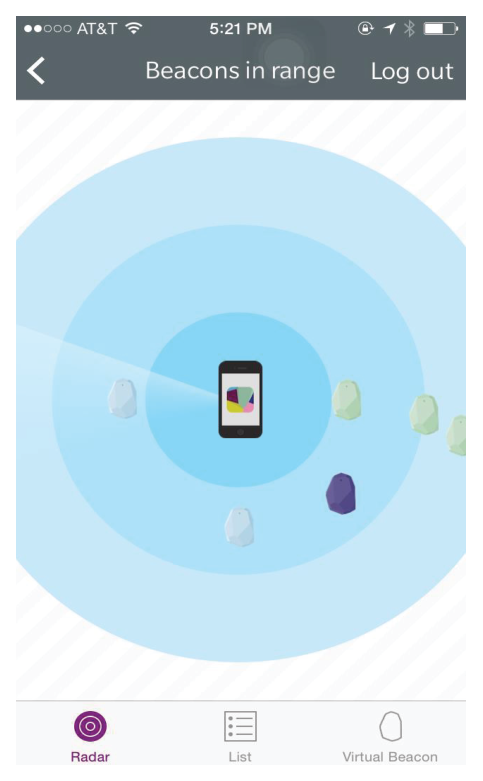
\includegraphics[width = 1\textwidth]{pictures/3_9a.eps}
		\end{minipage}
	}
	\subfigure[]{
		\begin{minipage}[htb]{0.25\textwidth}
			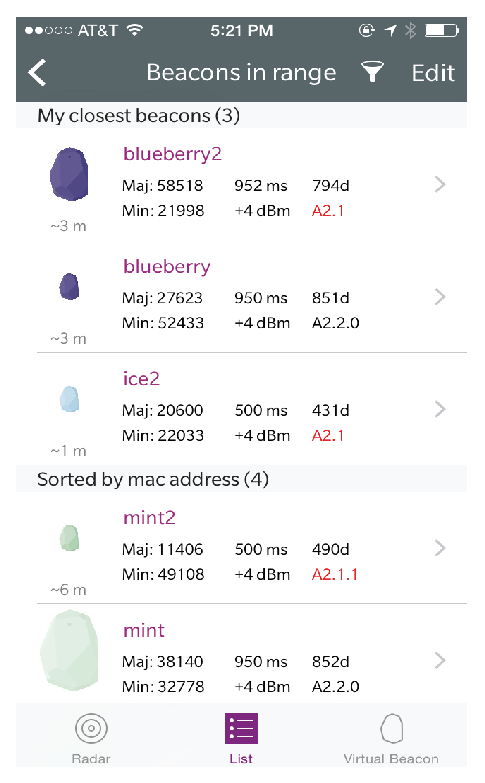
\includegraphics[width = \textwidth]{pictures/3_9b.eps}
		\end{minipage}
	}
	\subfigure[]{
		\begin{minipage}[htb]{0.25\textwidth}
			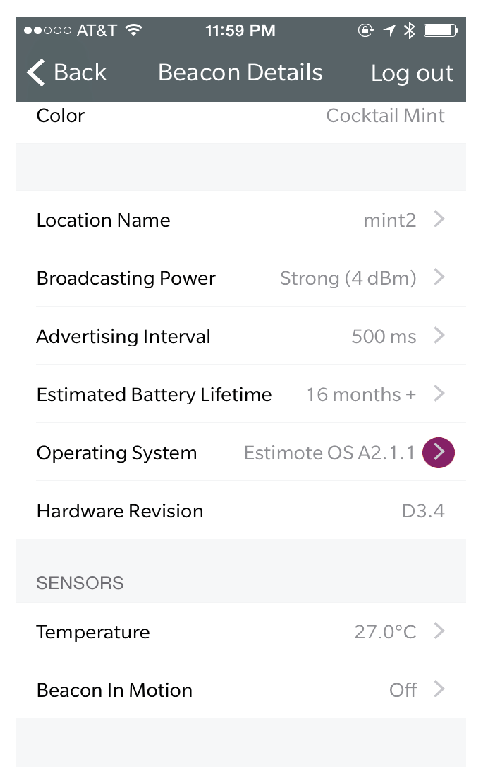
\includegraphics[width = \textwidth]{pictures/3_9c.eps}
		\end{minipage}
	}
	\caption{Typical screenshots of APP provided by Estimote.}
	\label{fig: 3.9}
\end{figure}

The manufacturer of iBeacon, Estimote company, provides their own iBeacon APP, which serves as a proximity estimator. The APP presents a graphic user interface (GUI) to display the geometric relationship between the iPhone and surrounding iBeacons. It also provides iBeacon ID, iBeacon status, distance between iBeacon and iPhone, iBeacon sensor reading and other information. 

Typical screenshot of this Estimote APP has been depicted in Figure~\ref{fig: 3.9}. It is very obvious that the Estimote APP has two major disadvantages considering the purpose of this paper. (1) Originally the APP is not designed to perform presence detection; (2) The APP fails to explicitly provide the RSSI reading. Given those disadvantages, it is necessary to design our own APP to achieve intelligent in-room presence detection.

To achieve in-room presence detection, we have to design our own APP. Since intuitively we know that the geometric relationship between the iBeacon and iPhone can be reflected by the RSSI fluctuation of beacon signal, we employ necessary APIs to get the RSSI reading directly from iPhone sensors. The APP encapsulates three essential information into each record, including the iBeacon ID, RSSI reading and Time stamp. Considering the scalability of the system, iBeacon ID has been partitioned into Universally Unique Identifier (UUID), Major field, and Minor field. In that sense, for large scale deployment, we may configure building number as iBeacon UUID, floor number as iBeacon Major and the iBeacon indicator as iBeacon Minor. The structure of each record can be given as
$$\{UUID, Major, Minor, RSSI, Time stamp\}$$

Typical screenshot of our own APP has been depicted in Figure~\ref{fig: 3.10}, in which we explicitly display Major, Minor and RSSI fields but implicitly record the UUID and Time stamp for privacy concerns.

\begin{figure}[htb]
	\begin{center}
		\begin{tabular}{c}
			\scalebox{0.5}{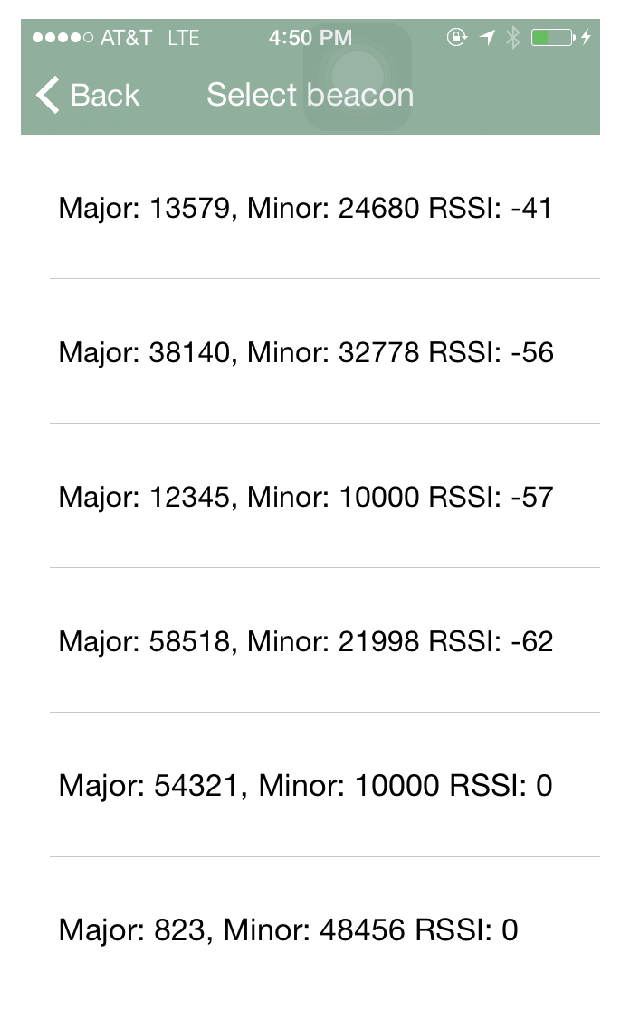
\includegraphics[]{pictures/3_10.eps}}
		\end{tabular}
	\end{center}
	\caption{Typical screenshot of our self-designed APP.}
	\label{fig: 3.10}
\end{figure}

\section{Presence Detection Algorithms}
Our self-designed APP is written in Objective-C and has been tested with iPhone 5s and all newer versions. The APP firstly collects iBeacon RSSI readings upon activation and then sends the records to a remote server over wireless connection. Throughout the experiments, a Macbook has been employed to provide server side calculation and count the number of presences. The server side functionalities are implemented in Python. 



\subsection{Double iBeacon Approach}

In order to implement the double iBeacons in-room presence detection system, it is necessary to clarify three distinguished movements of the Mobile Holder1 (MH). The first type of movement is represented by yellow arrows in Fig~\ref{fig: 3.11}. The MH is walking pass the entrance of the room without opening the door or entering. This is the most frequently appeared situation. The second type of movement is depicted by blue arrows, for which the MH is walking into the room. The third type of movement is represented by red arrows, for which the MH is going out of the room. The goal of your approach is to distinguish those three types of movements and properly adjusts the counter whenever there is a MH going into or out of the room.

\begin{figure}[htb]
	\begin{center}
		\begin{tabular}{c}
			\scalebox{0.9}{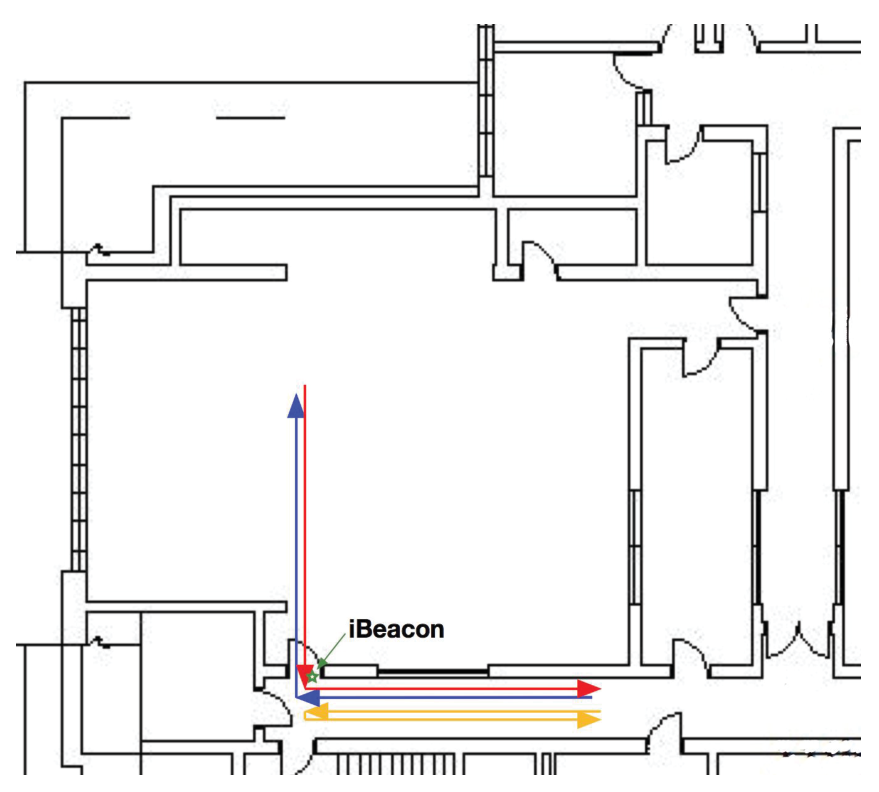
\includegraphics[]{pictures/3_11.eps}}
		\end{tabular}
	\end{center}
	\caption{Experimental environment and three different types of movements.}
	\label{fig: 3.11}
\end{figure}

The RSSI recording process is initiated by the motion sensor reading from iBeacon whenever the door is open. Any MH in the iBeacon coverage will be triggered to start data recording at a sample rate of 10Hz until it gets terminated by another iBeacon motion sensor reading showing that the door is closed again. When the recording process finishes, the APP uploads recorded data to the server in a binary file. The detailed logic for the self-designed APP has been shown in Algorithm 1.

\begin{algorithm}[!htp]
  \caption{Logic for the self-designed APP}
  \begin{algorithmic}[1]
  \vspace{3mm}
    \State $\textbf{Initialize}$ motion sensor $\textbf{status}$ as ``closed'';
    \vspace{3mm}
    \State $\textbf{while}$ ($\textbf{status}$==``closed'')
    \vspace{3mm}
		\State $\hspace{3mm}$ Monitor and update motion sensor $\textbf{status}$;
		\vspace{3mm}
		\State $\hspace{3mm}$ $\textbf{while}$ ($\textbf{status}$==``open'');
		\vspace{3mm}
		\State $\hspace{8mm}$ Record $\textrm{RSSI}_\textrm{out}$ and $\textrm{RSSI}_\textrm{in}$;
		\vspace{3mm}
		\State $\hspace{8mm}$ Monitor and update motion sensor $\textbf{status}$;
		\vspace{3mm}
		\State $\hspace{8mm}$ $\textbf{if}$ ($\textbf{status}$==``closed'')
		\vspace{3mm}
		\State $\hspace{12mm}$ Send RSSI records to server;
		\vspace{3mm}
		\State $\hspace{8mm}$ $\textbf{end}$
		\vspace{3mm}
		\State $\hspace{3mm}$ $\textbf{end}$
		\vspace{3mm}
		\State $\textbf{end}$
		\vspace{3mm}
  \end{algorithmic}
\end{algorithm}

\begin{algorithm}[!htp]
  \caption{Logic for the server}
  \begin{algorithmic}[1]
  \vspace{3mm}
    \State $\textbf{foreach}$ iBeacon ID, $\textbf{do}$
    \vspace{3mm}
    \State $\hspace{3mm}$ Acquire RSSI info from file;
    \vspace{3mm}
		\State $\hspace{3mm}$ $\textbf{label}_\textbf{out}$ = false; //Initialization
		\vspace{3mm}
		\State $\hspace{3mm}$ $\textbf{label}_\textbf{in}$ = false;
		\vspace{3mm}
		\State $\hspace{3mm}$ $\textbf{origin}$ = ($\textrm{RSSI}_{\textrm{out},t=1} > \textrm{RSSI}_{\textrm{in},t=1}$)?true:false;
		\vspace{3mm}
		\State $\hspace{3mm}$ $\textbf{for}$ $t$ = 1 to N, $\textbf{do}$; // Traverse by time stamp
		\vspace{3mm}
		\State $\hspace{8mm}$ $\textbf{if}$ ($\textrm{RSSI}_{\textrm{out},t}$ - $\textrm{RSSI}_{\textrm{in},t}$ $\geq$ 3) 
		//3dB RSSI threshold
		\vspace{3mm}
		\State $\hspace{12mm}$ $\textbf{label}_\textbf{out}$ = true; 
		//MH has appeared outside room
		\vspace{3mm}
		\State $\hspace{8mm}$ $\textbf{end}$
		\vspace{3mm}
		\State $\hspace{8mm}$ $\textbf{if}$ ($\textrm{RSSI}_{\textrm{out},t}$ - $\textrm{RSSI}_{\textrm{in},t}$ $\leq$ -3) 
		\vspace{3mm}
		\State $\hspace{12mm}$ $\textbf{label}_\textbf{in}$ = true; 
		//MH has appeared inside room
		\vspace{3mm}
		\State $\hspace{8mm}$ $\textbf{end}$
		\vspace{3mm}
		\State $\hspace{3mm}$ $\textbf{end}$
		\vspace{3mm}
		\State $\hspace{3mm}$ $\textbf{if}$ ($\textbf{label}_\textbf{out} \cap \textbf{label}_\textbf{in}$) 
		//MH goes through the door
		\vspace{3mm}
		\State $\hspace{8mm}$ $\textbf{type} = (\textbf{origin})$?-1:1; 
		// 1 for enter, -1 for leave
		\vspace{3mm}
		\State $\hspace{8mm}$ $\textbf{counter} = \textbf{counter}+\textbf{type}$; 
		// \# people in-room
		\vspace{3mm}
		\State $\hspace{3mm}$ $\textbf{end}$
		\vspace{3mm}
		\State $\textbf{end}$
		\vspace{3mm}
  \end{algorithmic}
\end{algorithm}

\begin{figure}[htb]
	\begin{center}
		\begin{tabular}{c}
			\scalebox{0.9}{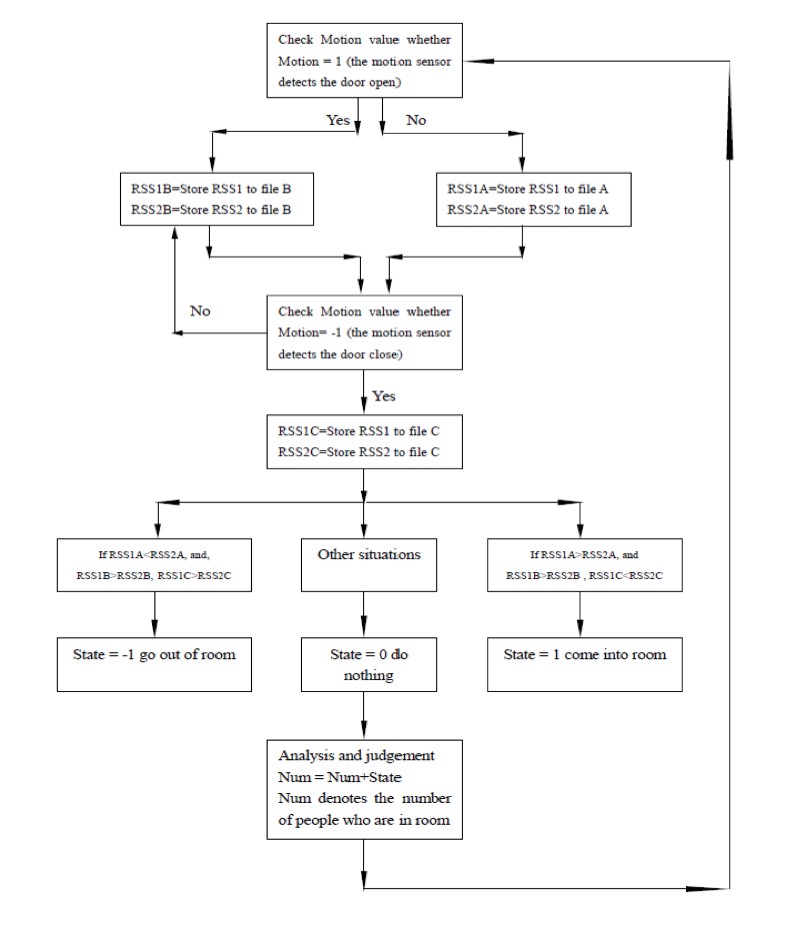
\includegraphics[]{pictures/34.eps}}
		\end{tabular}
	\end{center}
	\caption{Experimental environment and three different types of movements.}
	\label{fig: 3.4}
\end{figure}

Since we attach one of the iBeacon to a specific side of the door and another iBeacon to the same position on the other side, the path-loss between each iBeacon and the iPhone is supposed to be different. Such path-loss difference is caused by the wooden/metallic door (and surrounding walls), which is lossy medium for radio propagation. We denote RSSI reading of the two iBeacons as RSSIout for outside iBeacon and RSSIin for inside iBeacon, so that the server side can easily determine the MH movements by the logic shown in Algorithm 2. The flow chart of the algorithm is shown in Fig~\ref{fig: 3.4}.The performance of double iBeacon approach will be investigated in the following sections.




\subsection{Single iBeacon Approach}
Even though iBeacons are considerably cheap, less iBeacons still guarantee lower cost and more convenience. We believe it is reasonable to take efforts and improve our system to the single iBeacon implementation. As is mentioned in previous sections, that scenario requires the assumption that the en- trance door will be kept closed, that is, an individual will always shut the door no matter he/she goes into or out of the room. That assumption most frequently holds when the door automatically shuts. Given the assumption of this work, we know that the individual needs to be near the door and touch the knob to have it open, which results in a spike of RSSI reading. In that sense, the presence detection can be regarded as a RSSI value peak detection with properly setting thresholds. Based on that idea, we propose the single iBeacon system block diagram in Fig~\ref{fig: 3.12}. Note that for single iBeacon approach, the iBeacon is attached to the outside of the entrance door near the knob. 

\begin{figure}[htb]
	\begin{center}
		\begin{tabular}{c}
			\scalebox{0.8}{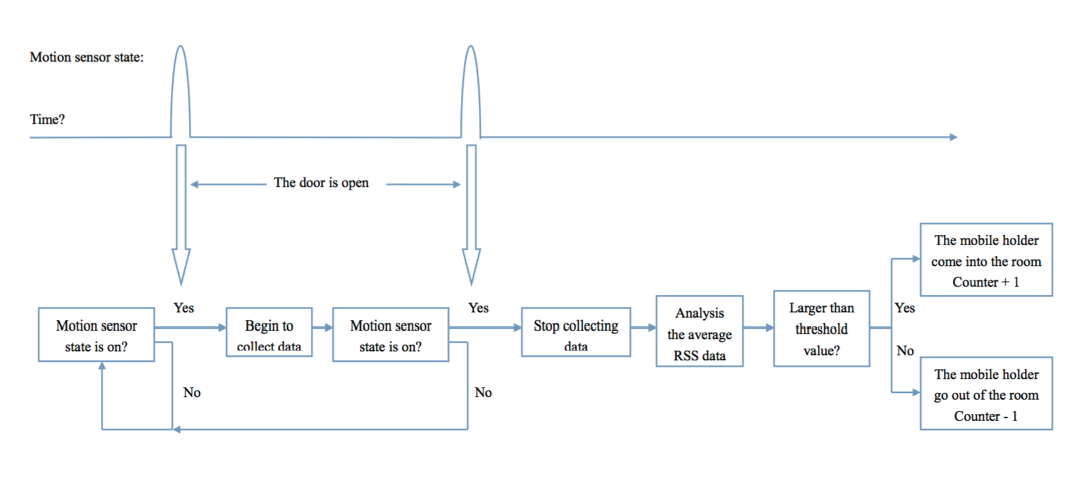
\includegraphics[]{pictures/3_12.eps}}
		\end{tabular}
	\end{center}
	\caption{Experimental environment and three different types of movements.}
	\label{fig: 3.12}
\end{figure}

The logic for APP side is almost identical to the double iBeacons approach except for the fact that we only record and upload the RSSI information of the only single iBeacon. At the server side, we still use the iBeacon motion sensor status as the trigger and terminator of RSSI recording process. Within the activate sampling period, the server first and foremost performs a pick detection and then uses -60dB RSSI as the threshold to determine whether the MH is leaving or entering the room. For the case with maximum RSSI greater than - 60dB, the MH is entering the room, otherwise, the MH is leaving the room. The selection of -60dB threshold comes from the analysis of empirical data and the threshold only works for the scenarios that iBeacon is attached to the outside of the entrance door.


\section{Performance Evaluation}
In this section we validate the proposed systems. Each previously mentioned movement has been repeated for over 500 times and the RSSI of iBeacons has been measured. By investigating the RSSI samples, we show the validity of our approach using physical observation. Apart from that, the system performance has been also recorded to help the performance comparison between double and single iBeacon approaches. 

\begin{figure}[htb]
	\begin{center}
		\begin{tabular}{c}
			\scalebox{0.65}{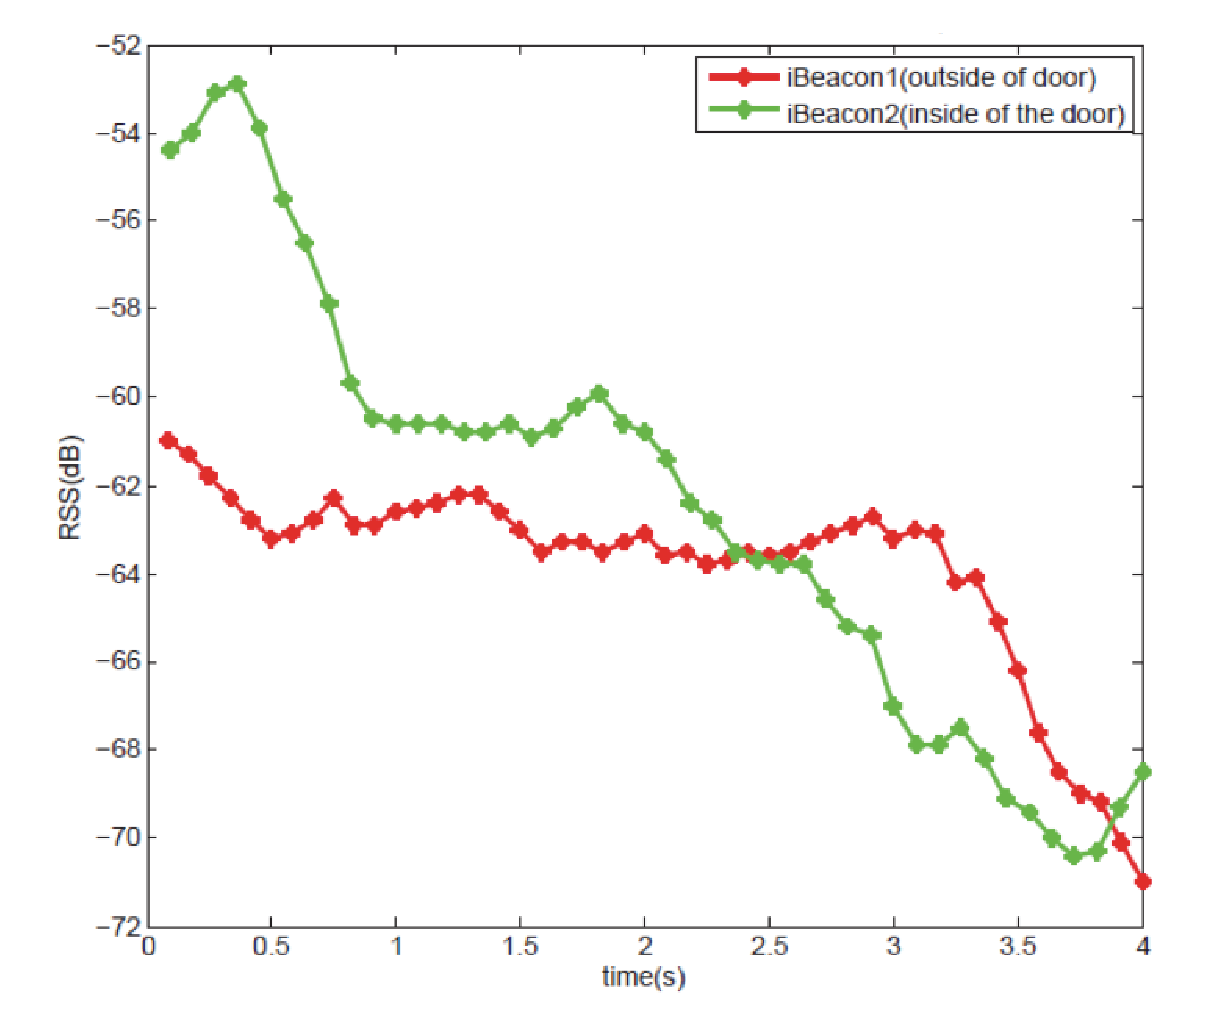
\includegraphics[]{pictures/3_13.eps}}
		\end{tabular}
	\end{center}
	\caption{RSSI vs Time in Double iBeacon Leaving Scenario.}
	\label{fig: 3.13}
\end{figure}

The RSSI samples for typical leaving movement have been plotted in Fig~\ref{fig: 3.13}. As shown in the figure, when the MH opens the door, iBeacon 2 (on inside door) provides -54dB RSSI while iBeacon 1 (on outside door) has only -61dB. With the time going, when MH goes through the door at t = 2.5s, both iBeacons show approximately 63.5dB RSSI. After that, when the MH gets out of the room, the two RSSI curves flip over and iBeacon 1 dwells on top of iBeacon 2. As for typical entering movement, the opposite trend can be found, which still shows that the double iBeacons approach can provide successful detection. One thing worth mentioning is that we also investigated the situation that a MH came, open the door and then closed it without entering or leaving the room. The RSSI curve for that movement has been plotted in Fig~\ref{fig: 3.14}.

\begin{figure}[htb]
	\begin{center}
		\begin{tabular}{c}
			\scalebox{0.65}{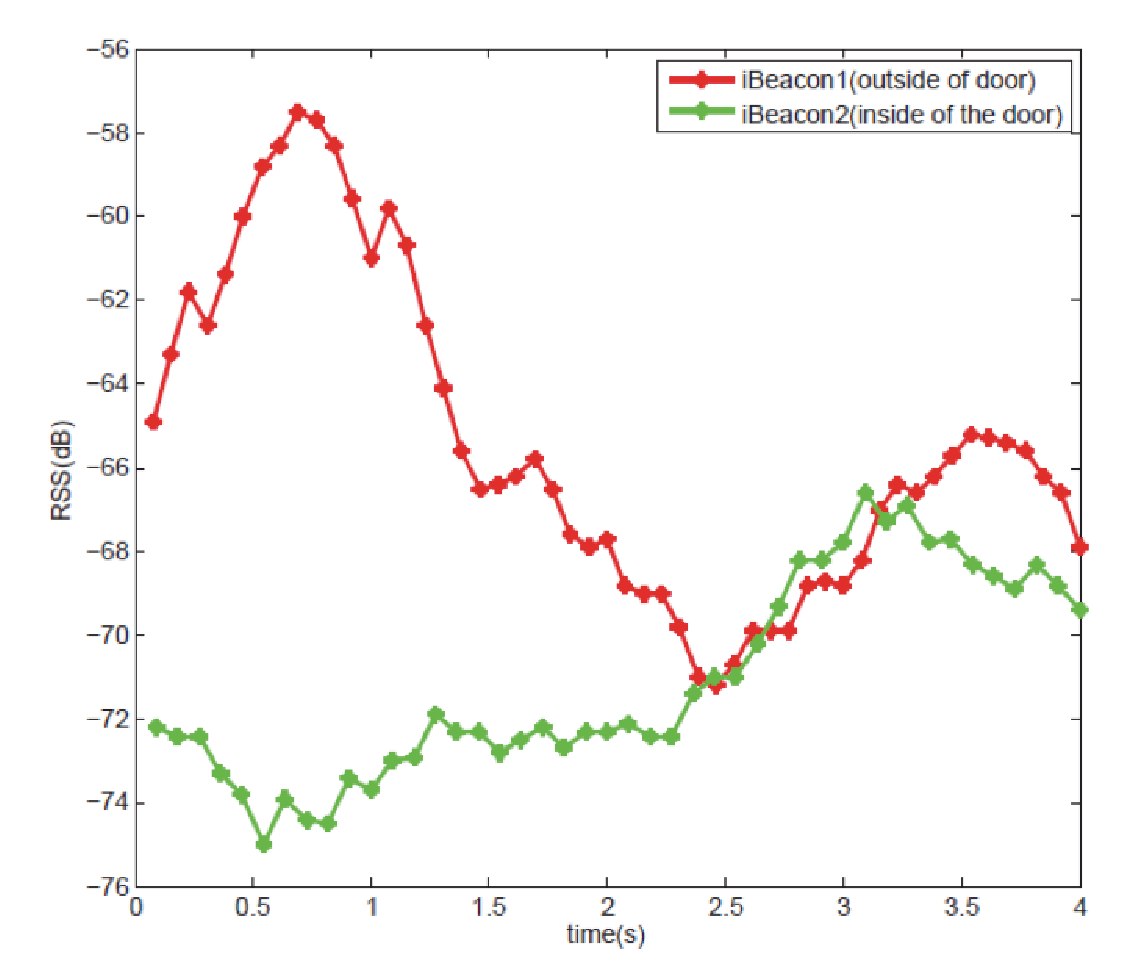
\includegraphics[]{pictures/3_14.eps}}
		\end{tabular}
	\end{center}
	\caption{RSSI vs Time in Double iBeacon Passing Scenario.}
	\label{fig: 3.14}
\end{figure}

Given that the double iBeacons approach performs well, we move on to the validation of single iBeacon approach. Among our 1536 sets of empirical data, the typical cases for entering and leaving the room have been plotted in Fig~\ref{fig: 3.15}. It is clear that entering the room results in higher RSSI peak due to the fact that the single iBeacon is attached to the outside of the door. When the MH is in the room, even though he/she could be close to the iBeacon, but the door lies between iBeacon and iPhone can create extra path-loss. The choice of -60dB RSSI threshold comes from the regression fitting of our empirical data, that is, we find the best fit curves for both entering and leaving movements and notice that -60dB threshold provides satisfactory detection rate of different movements. To guarantee the robustness of the single iBeacon approach, we also conduct experiments with the iPhone located at various positions. In hand, pant pocket and shirt pocket have been selected as candidate locations of the iPhone and the best fit RSSI curves have been plotted in Fig~\ref{fig: 3.16}, respectively. Clearly we know that -60dB threshold works for all those iPhone positions. 

\begin{figure}[htb]
	\begin{center}
		\begin{tabular}{c}
			\scalebox{0.65}{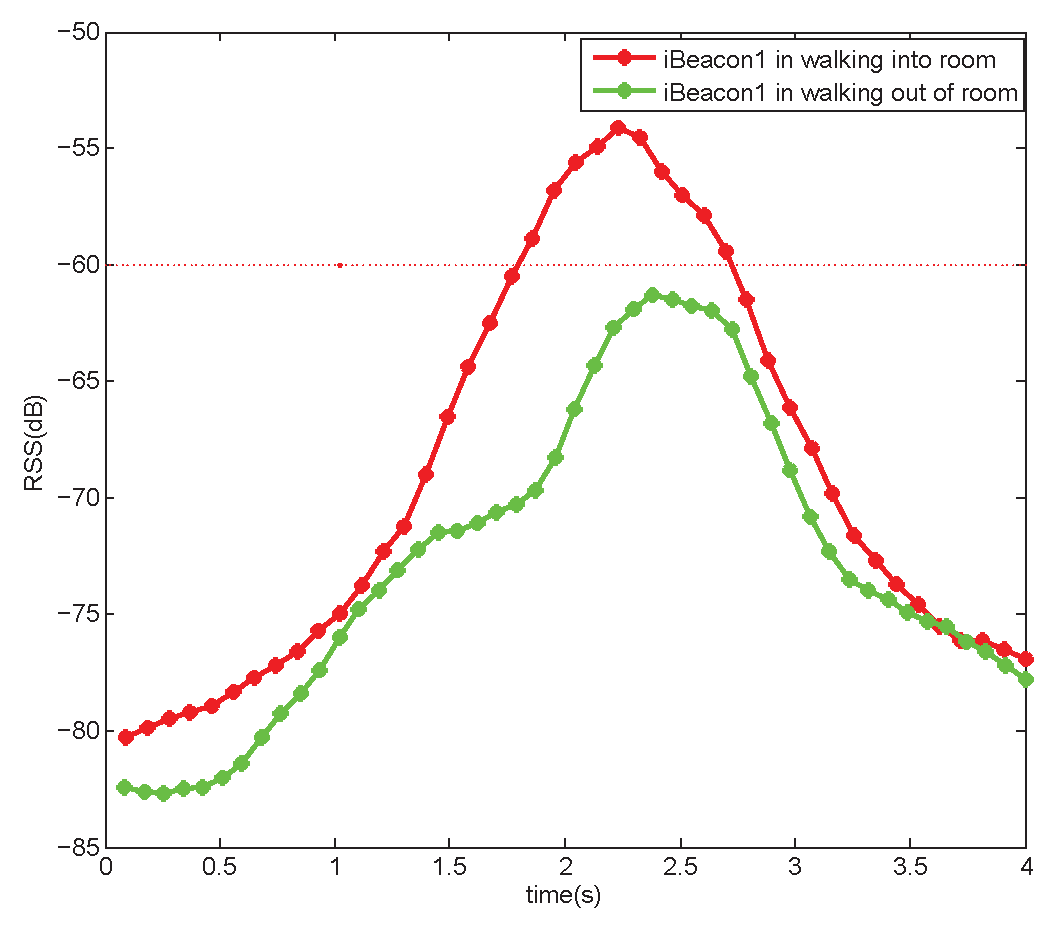
\includegraphics[]{pictures/3_15.eps}}
		\end{tabular}
	\end{center}
	\caption{RSSI vs Time in Single iBeacon Entering and Leaving Scenario.}
	\label{fig: 3.15}
\end{figure}

\begin{figure}[htb]
	\begin{center}
		\begin{tabular}{c}
			\scalebox{0.65}{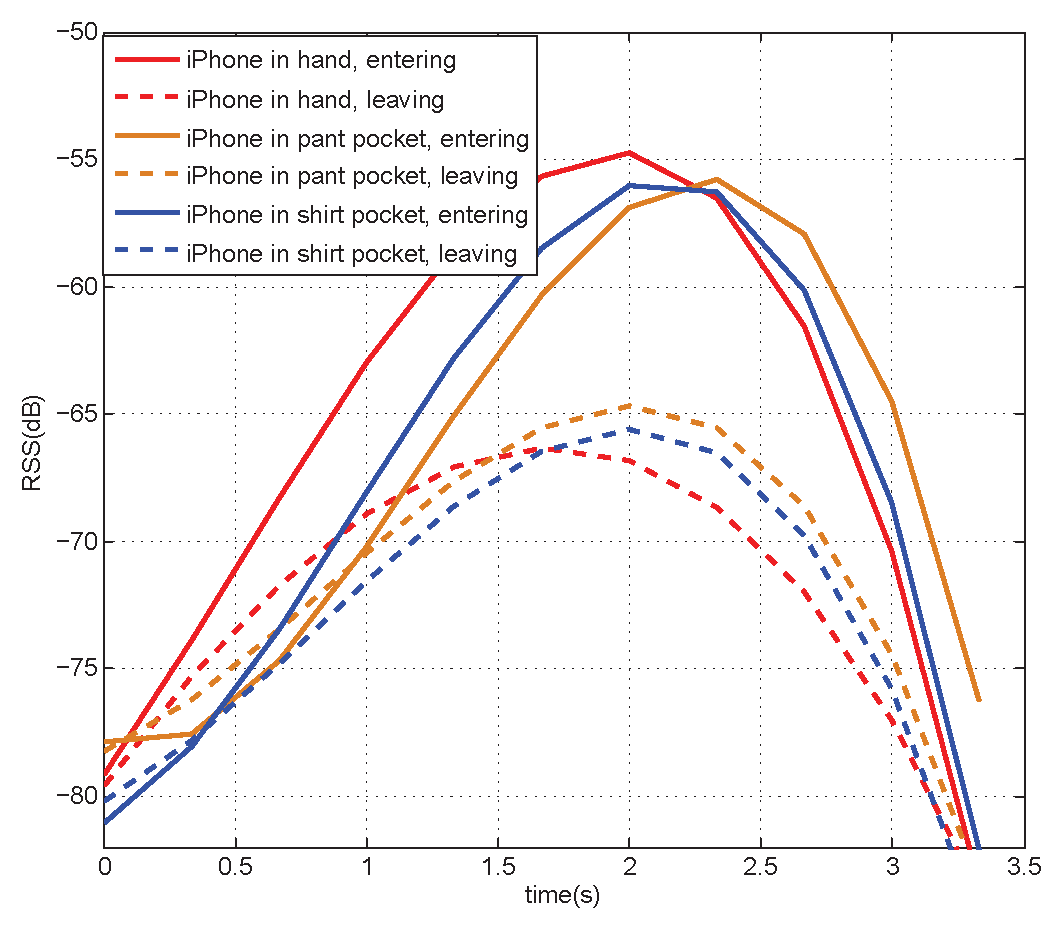
\includegraphics[]{pictures/3_16.eps}}
		\end{tabular}
	\end{center}
	\caption{Comparison of Single iBeacon Approach in Different Scenarios.}
	\label{fig: 3.16}
\end{figure}

It is worth mentioning that the single iBeacon approach is not able to detect the situation that the MH opens the door but neither entering nor leaving the room. Such reality shows that the single iBeacon is cost effective compared with double iBeacons approach, but is less robust against outliers.


\section{Results and Discussions}
At the end of this part, we would like to discuss the detection rates of the proposed systems. For the double iBeacons approach, we performed 521 measurements with the MH holding iPhone in hand, 500 measurements with the MH putting iPhone in pant pocket and another 500 measurements with iPhone in shirt pocket. For all these measurements, the double iBeacons approach is able to correctly detect the in-room presence. As for single iBeacon approach, we have 536 measurements with the MH holding iPhone in hand, 500 measurements with the MH putting iPhone in pant pocket and another 500 measurements with iPhone in shirt pocket. For the pant pocket iPhone position we have 2 mis-detections, while for in hand and shirt pocket cases the detection rates are all 100\%. With such experimental results, we would like to claim that both approaches work well.

\begin{table}[!htp]
\begin{center}
\caption{Performance of proposed in-room presence detection approaches.} 
\begin{tabular}[b]{ c || c c c}
	\hline
	\hline
	$\textbf{Implementation}$	& $\textbf{iPhone}$   & $\textbf{Detection}$ & $\textbf{Detection}$\\
	$\textbf{approaches}$ & $\textbf{position}$ & $\textbf{rate}$      & $\textbf{rate (\%)}$\\
  \hline
	Double iBeacon 	& any						& 1521/1521 & 100\% \\
	\hline								
									& in hand 			& 500/500		& 100\% \\
	Single iBeacon	& pant pocket 	& 534/536		& 99.63\% \\
									& shirt pocket	& 500/500		& 100\% \\
	\hline
	\hline
\end{tabular}
\end{center}
\vspace{-6mm}
\end{table}

Since both of the two algorithms reach the detection rate of almost 100\% accuracy, we can say that they are reliable for distinguishing the basic scenerios of human movement and can be used to build the iBeacon based intelligent in-room
presence detection system. Since single iBeacon approach needs one less iBeacon on each door than double iBeacon approach and the algorithm is relatively simpler, we think single iBeacon approach is adequate for practice.

In this part, we investigated and developed an iBeacon based intelligent in-room presence detection system to record the users in a room. We collected the RSSI data of iBeacon for LOS situation in a typical indoor office environment and we implement both single beacon and double beacons based approach. We also analyzed the probability density function, error detection rate and other metrics using the empirical mea- surement results. The optimal performance of our approach can be as high as 100\%.

%%%%%%%%%%%%%%%%%%%%%%%%%%%%%%%%%%%%%%%%%%%%%%%%%%%%%%%%%%%%%%%%%%%%%%%%%%%%%%%%%%%%%%
%%%%%%%%%%%%%%%%%%%%%%%%%%%%%%%%%%%%%%%%%%%%%%%%%%%%%%%%%%%%%%%%%%%%%%%%%%%%%%%%%%%%%%
%%%%%%%%%%%%%%%%%%%%%%%%%%%%%%%%%%%%%%%%%%%%%%%%%%%%%%%%%%%%%%%%%%%%%%%%%%%%%%%%%%%%%%
%										Chapter 4
%%%%%%%%%%%%%%%%%%%%%%%%%%%%%%%%%%%%%%%%%%%%%%%%%%%%%%%%%%%%%%%%%%%%%%%%%%%%%%%%%%%%%%
%%%%%%%%%%%%%%%%%%%%%%%%%%%%%%%%%%%%%%%%%%%%%%%%%%%%%%%%%%%%%%%%%%%%%%%%%%%%%%%%%%%%%%
%%%%%%%%%%%%%%%%%%%%%%%%%%%%%%%%%%%%%%%%%%%%%%%%%%%%%%%%%%%%%%%%%%%%%%%%%%%%%%%%%%%%%%

\chapter{Path-loss Modeling and Performance of In-Room Localization}
In this chapter, we introduce our data collecting system based on which we do RSSI measurements and derive the reality path-loss model. Then we compare the performance of that model and existing iBeacon model by the CDF of DME to reach the conclusion that our reality path-loss model is more reliable. The path-loss model is used in the iBeacon based newborns localization system in hospitals. This part is lead by him. The details of the algorithms is written in my partner Yang Yang's thesis.

As mentioned in previous section, the iBeacons produced by Estimote company can provide us much information we need such as RSSI, broadcasting interval, minor and major values and even motion sensor. However, the existing app from Extimote company do not allow us to collect data directly from iphone which means large samples are impossible and we can only collect data by hand. To solve this problem, we decide to develop our own app.

We use Objective-C to develop our app to get the RSSI of the beacons. The iPhone 5s acts as the receiver in our research and it is connected to a Mac book computer by a cable. When it gets the packets from iBeacons which are in the detection range, it will display the current values of RSS both on the iPhone screen and Mac book computer. The data we collected in different situation can be used to do the channel modeling. 

The achievements of our developing own app:\\
1. Connect with certain iBeacon.\\
2. Set the UUID, major and minor fields of iBeacon.\\
3. Collect and store the RSS information.\\
4. Extract the RSS data from iphone. This makes the data more reliable compared with those collected by hand, and also make the samples much larger.

\section{Modern RF Based In-Room Localization}
With the heating up of the indoor localization for years, plenty of corresponding technologies have been developed and some of them have been implemented. They all have their unique advantages and limitations. Almost all of them can be divided into three categories according to the technologies they use. There are two primary options for RF-based localization: WiFi Positioning System (WPS) and Ultra-wide Band (UWB). Each of them has already been applied widely and exposed some problems. 

\subsection{WiFi Positioning System}
Many works have been done on the WPS. In paper [Indoor WIFI localization on mobile devices], they discuss the performance of multi-trilateration and fingerprinting localization techniques in the context of mobile applications. The implementation of WIFI localization on mobile allows the users with WIFI-enable devices such as smartphone to locate their position and/or navigate themselves within the building. During their experiments, they noted that the selection criteria that involves selecting available access points to be used as a reference position considerably affect the accuracy of the positioning calculation. The tradeoff between multi-trilateration and fingerprinting in terms of correctness, computational complexity and system resource consumption have been discussed. Additionally, they proposed the suitable configuration for these localization algorithms as a means to achieve more accurate positioning results.

In paper [WiFi localization and navigation for autonomous indoor mobile robots], they contribute a mobile robot that autonomously navigates in indoor environments using WiFi sensory data. They model the world as a WiFi signature map with geometric constraints and introduce a continuous perceptual model of the environment generated from the discrete graph-based WiFi signal strength sampling. They contribute our WiFi localization algorithm which continuously uses the perceptual model to update the robot location in conjunction with its odometry data. They then briefly introduce a navigation approach that robustly uses the WiFi location estimates. They present the results of our exhaustive tests of the WiFi localization independently and in conjunction with the navigation of our custom-built mobile robot in extensive long autonomous runs. 

In the paper [Compressive Sensing Based Positioning Using RSS of WLAN Access Points], they address the received signal strength (RSS)-based localization problem in WLANs using the theory of compressive sensing (CS), which offers accurate recovery of sparse signals from a small number of measurements by solving an ¿1-minimization problem. A preprocessing procedure of orthogonalization is used to induce incoherence needed in the CS theory. In order to mitigate the effects of RSS variations due to channel impediments, the proposed positioning system consists of two steps: coarse localization by exploiting affinity propagation, and fine localization by the CS theory. In the fine localization stage, access point selection problem is studied to further increase the accuracy. They implement the positioning system on a WiFi-integrated mobile device (HP iPAQ hx4700 with Windows Mobile 2003 Pocket PC) to evaluate the performance. Experimental results indicate that the proposed system leads to substantial improvements on localization accuracy and complexity over the widely used traditional fingerprinting methods.

There are a lot of advantages of WiFi Positioning System. One of the most obvious one is about the infrastructure. Almost every place where position information may be required, such as campus, office, mall, and home, has already deployed routers. This gives us so much convenience to develop a system based on WiFi. However, the disadvantages are also obvious. Since the routers are for private use, they can be changed or even moved without notificatons. That is a heavy burden for the maintenance of the database for localization.

\subsection{Ultra-wide Band}
Ultra-wide band (UWB) is a radio technology pioneered by Robert A. Scholtz and others which may be used at a very low energy level for short-range, high-bandwidth communications using a large portion of the radio spectrum [UWB founded wiki]. UWB is a technology for transmitting information spread over a large bandwidth, lager than 500MHz. UWB has many applications including noncooperative radar imaging, sensor data collection, precision locating and tracking applications. Ultra wideband was formerly known as ”pulse radio”, but the FCC and the International Telecommunication Union Radio communication Sector (ITUR) currently define UWB in terms of a transmission from an antenna for which the emitted signal bandwidth exceeds the lesser of 500 MHz or 20\% of the center frequency. Thus, pulse-based systemswhere each transmitted pulse occupies the UWB bandwidth (or an aggregate of at least 500 MHz of narrow-band carrier; for example, orthogonal frequency-division multiplexing (OFDM)can gain access to the UWB spectrum under the rules. Pulse repetition rates may be either low or very high. Pulse-based UWB radars and imaging systems tend to use low repetition rates (typically in the range of 1 to 100 megapulses per second). On the other hand, communications systems favor high repetition rates (typically in the range of one to two gigapulses per second), thus enabling short-range gigabit-per-second communications systems. Each pulse in a pulse-based UWB system occupies the entire UWB bandwidth (thus reaping the benefits of relative immunity to multipath fading, but not intersymbol interference), unlike carrier-based systems which are subject to deep fading and intersymbol interference.

In paper [Mobile robot self-localization system using IR-UWB sensor in indoor environments], they propose the use of a new type of sensor that permits accurate localization in indoor environments. An impulse radio (IR) ultra wide-band (UWB) sensor uses very short baseband pulses for transmission. This sensor facilitates the development of indoor location and tracking applications based on time of arrival estimation with great accuracy. There are many different sensors and techniques that have been proposed for indoor localization; however they usually have large errors in non line of sight (NLOS) conditions or with certain environment conditions. The objective of this paper is to propose a self-localization system based on time of arrival (TOA) estimation algorithm that permits precise localization in indoor environments with obstructed line of sight. This work proposes a new wavelet cyclic cross correlation strategy for time of arrival estimation based on non-coherent receiver structure and sliding correlation techniques for multiple user differentiation. The simulation results show that the propose localization system overcome the problems of NLOS conditions and makes possible the mobile robot localization with small number of base stations.

\section{Path-loss Modeling of iBeacon}
For both the RSS based WiFi localization system and the TOA based UWB localization system, it is necessary to understand and statitically model the behavior of the radio propagation channel between the transmitter and receiver. There are many existing channel models in the open literature. Some of them come from research institutions and specific measurement campaigns, while others are proposed by standardization committees. Since the iBeacon based in-room localization system is RSS based, it is necessary to investigate the path-loss model for the Bluetooth channel. 

\subsection{Modeling and Validation}
Before we start to collect data, we need to validate the measurement environment can use the IEEE 802.11 model or not. Since RSS is the most important factor in this project, the path-loss model must be established. We do linear match fitting with different iBeacon data collected by out app to try to find out the best path-loss model of iBeacon. Distance measure error (DME) is the criterion we use to compare the performance of each model. The CDF of DME of different can tell us which model is better.

With the data we collected, here is the path-loss model in LOS situation for RSS based ranging. After linear match fitting with the RSS, we have figure below which shows us the power gradient and the pass-loss in first meter.

In order to find out how Estimote company measure the distance by iBeacon, we recorded the RSS data shown in Estimote app when the app indicated we were on the boundaries of first and second circles(distances are 1m and 5m). With the RSS data of these two points, we can figure out the path-loss model using by iBeacon. We have two path-loss models for each iBeacon coming from Estimote company and our own app, we can see that there are some differences between these two models as shown in Fig~\ref{fig: 4.1}.

\begin{figure}[htb]
	\begin{center}
		\begin{tabular}{c}
			\scalebox{1.0}{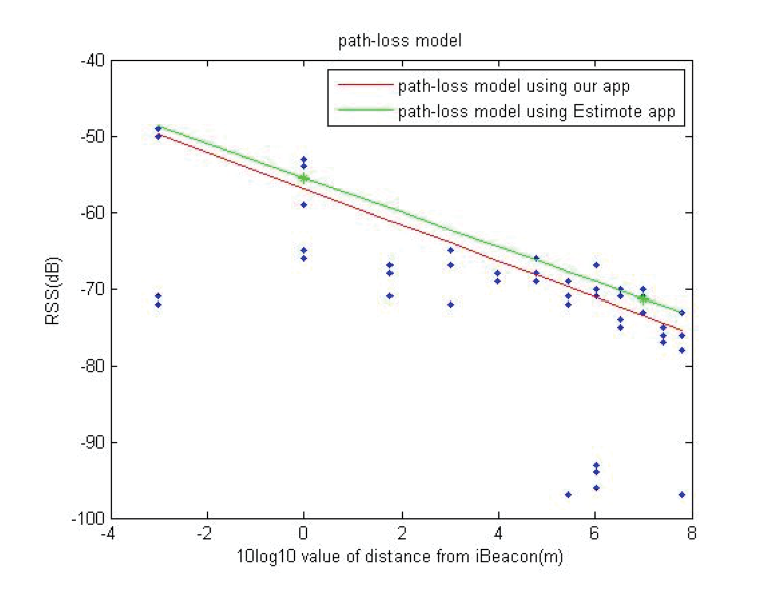
\includegraphics[]{pictures/4_1.eps}}
		\end{tabular}
	\end{center}
	\caption{Two Path-loss Models Comparison.}
	\label{fig: 4.1}
\end{figure}

With the data we collected by mint iBeacon, we can find out the estimate distance by using the RSS data and path-loss model. Both the estimote path-loss model and our path-loss model follow the similar formulation with the IEEE 802.11 SISO radio propagation model, which can be given as:

\begin{equation}
\textrm{RSSI}(\hat{d}) = P_r =\textrm{P}_t-\textrm{L}_p(d_0)-10\alpha\log_{10}\frac{d}{d_0}+\sigma_{SF}
\end{equation}

where $d$ denotes to the actual distance between the smart phone and a specific iBeacon, $\textrm{P}_t$ is the constant transmit power of iBeacons, $\textrm{L}_p(d_0)$ is the path-loss at reference distance $d_0$ (i.e. 1m in this work), $\alpha$ denotes to the distance-power gradient and $\sigma$ denotes to the shadow fading effect. the ranging estimate can be shown as

\begin{equation}
\hat{d}=10^{\left( \frac{\textrm{RSSI}(\hat{d})-\textrm{P}_t+\textrm{L}_{p}(d_0)}{10\alpha} \right)}\times d_0
\end{equation}

Then the DME can be shown as the difference between estimate distance $\hat{d}$ and actual distance $d$:
\begin{equation}
DME = |d - \hat{d}|
\end{equation}

where d is the real distance we have in measurement. We calculate the DME for each point data we have and then compute the CDF of the DME to compare the performance of these two models, the CDF of mint iBeacon is shown as Fig~\ref{fig: 4.2}.

\begin{figure}[htb]
	\begin{center}
		\begin{tabular}{c}
			\scalebox{1.0}{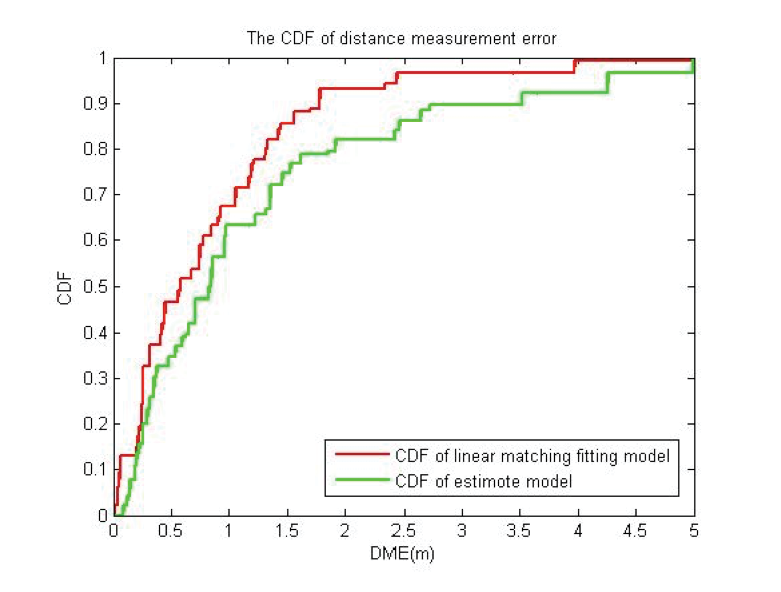
\includegraphics[]{pictures/4_2.eps}}
		\end{tabular}
	\end{center}
	\caption{Comparison of DME CDF.}
	\label{fig: 4.2}
\end{figure}

From the Fig~\ref{fig: 4.2} we can see that the red CDF is on the left side of green CDF which means our path-loss model coming from linear match fitting has less error in the same DME range. In a word, the linear match fitting path-loss model shows a better performance.

\subsection{Overall Path-loss Modeling Results}
In this part, different iBeacons have different path-loss model which may be caused by shadow fading or measurement error. However, after comparing the CDF of DME, our model coming from linear matching shows a better performance, using our model may have a better distance judgement. The overall two path-loss models are shown in table-1, where σSF(m) means the mean of shadow fading using each model.

\begin{table}[!htp]
\begin{center}
\caption{Performance of proposed in-room presence detection approaches.} 
\begin{tabular}[b]{ c || c | c | c || c | c | c}
	\hline
	\hline
	& \multicolumn{3} {c||} {$\textbf{Estimote iBeacon}$} 	& \multicolumn{3} {c} {$\textbf{Our own}$}  \\
	& \multicolumn{3} {c||} {$\textbf{path-loss model}$} 	& \multicolumn{3} {c} {$\textbf{path-loss model}$}  \\
	  	
  	\hline
	$\textbf{Characteristic}$ 	& $\textrm{L}_p(d_0)$ & $\alpha$ & $\sigma_{SF}$ & $\textrm{L}_p(d_0)$ & $\alpha$ & $\sigma_{SF}$ \\
	\hline								
	$\textbf{iBeacon 1}$ 		& 54.8995 & 2.5214 & 3.2013 & 55.3555 &	2.4674 & 3.5773 \\
	\hline
	$\textbf{iBeacon 2}$ 		& 55.5000 & 2.2540 & 4.2992 & 56.8918 &	2.3689 & 3.0501 \\
	\hline
	$\textbf{iBeacon 3}$ 		& 52.5628 & 2.7693 & 4.1208 & 56.1283 &	2.5387 & 3.1099 \\
	\hline
	\hline
\end{tabular}
\end{center}
\end{table}

Based on the models, we also calculate the DME of each model to decide which one owes a better performance, the comparison results are shown in table-2, where me(m) means the mean of DME using each model and σe(m) means the standard variance of DME using each model.

\begin{table}[!htp]
\begin{center}
\caption{Performance of proposed in-room presence detection approaches.} 
\begin{tabular}[b]{ c || c | c || c | c}
	\hline
	\hline
	& \multicolumn{2} {c||} {$\textbf{Estimote iBeacon}$} 	& \multicolumn{2} {c} {$\textbf{Our own}$}  \\
	& \multicolumn{2} {c||} {$\textbf{path-loss model}$} 	& \multicolumn{2} {c} {$\textbf{path-loss model}$}  \\
	  	
  	\hline
	$\textbf{Characteristic}$ 	& $\mu_e$ & $\sigma_e$ & $\mu_e$ & $\sigma_{e}$ \\
	\hline								
	$\textbf{iBeacon 1}$ 		& 0.8716 & 1.1819 & 0.8771 & 1.2179 \\
	\hline
	$\textbf{iBeacon 2}$ 		& 1.6717 & 4.9553 & 1.0788 & 1.4071 \\
	\hline
	$\textbf{iBeacon 3}$ 		& 0.1739 & 2.0837 & 0.9872 & 1.9240 \\
	\hline
	\hline
\end{tabular}
\end{center}
\end{table}

\section{Scenarios of In-Room Localization}
Ranging-based localization is the task of identifying the positions of a network of nodes based on estimates of the distances between them, called range estimates. In many ways, radio signal strength (RSS) is an ideal modality for range estimation in wireless networks because RSS information can be obtained at no additional cost with each radio message sent and received. The simplicity of RSS is especially appealing for the localization in wireless sensor networks because of their cost, size, and power constraints, despite the fact that RSS may yield very noisy range estimates. In this section, we empirically introduce the main methodology of RSS-based localization such we can have an overview of in-room localization using iBeacon.

\begin{figure}[htb]
	\begin{center}
		\begin{tabular}{c}
			\scalebox{1.4}{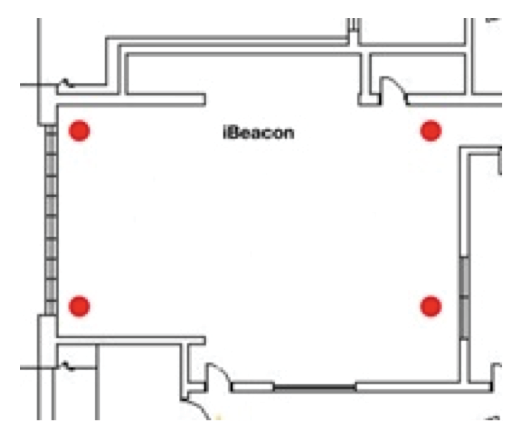
\includegraphics[]{pictures/4_3.eps}}
		\end{tabular}
	\end{center}
	\caption{Main Scenario of In-Room Localization.}
	\label{fig: 4.3}
\end{figure}

Fig~\ref{fig: 4.3} shows the main scenario for in-room localization that there are 4 iBeacons in each corner of a room.  This is a typical scenario that we usually consider it as our first choice. It is very similar to Wi-Fi localization if we regard the iBeacons as access points.

\begin{figure}[htb]
	\begin{center}
		\begin{tabular}{c}
			\scalebox{1.4}{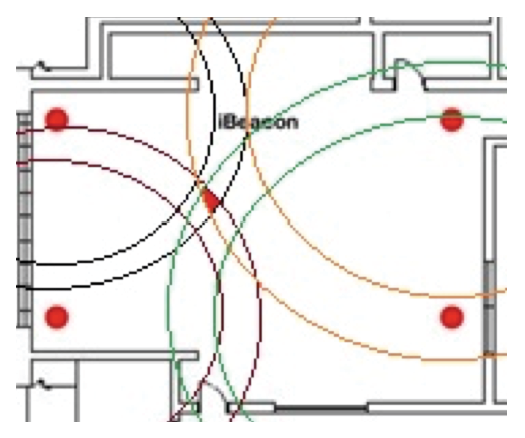
\includegraphics[]{pictures/4_4.eps}}
		\end{tabular}
	\end{center}
	\caption{Algorithm of In-Room Localization.}
	\label{fig: 4.4}
\end{figure}

To the localization in this room, we record the RSS data from all these 4 iBeacons, from each iBeacon RSS data we can calculate a distance range based on the path-loss model we construct in section 3.2. Then we use that distance range as radius range and take the location of each iBeacon as a center to draw circles. The overlap area shown in red shows the possible location we locate by iBeacon, shown in Fig~\ref{fig: 4.4}.


%%%%%%%%%%%%%%%%%%%%%%%%%%%%%%%%%%%%%%%%%%%%%%%%%%%%%%%%%%%%%%%%%%%%%%%%%%%%%%%%%%%%%%%%%%%%%%%%%%%%%%%%%%%%%%%%%%%%%

\section{Performance Evaluation}
In this part, we firstly introduce the scenarios we define to evaluate the performance of using iBeacon in localization. Then based on Matlab, we simulate the in-room localization environment and calculate the estimation of location error to show the effects of different deployment patterns and different iBeacon numbers. Furthermore, we promote our model from 2D to 3D scenario and figure out the estimation of location error to present the feasibility in this case.

\subsection{Evaluation Scenario}
In order to compare the performance of different localization methods, in this paper we use Cramér-Rao low bound of the location error standard deviation as the assessment criterion. According to the conclusion given in Signal Strength Based Indoor Geolocation [1], we know how to calculate the location error standard deviation. We use Matlab simulation to obtain the theoretic results.

\begin{figure}[htb]
	\begin{center}
		\begin{tabular}{c}
			\scalebox{0.5}{\includegraphics[]{pictures/5_5.eps}}
		\end{tabular}
	\end{center}
	\caption{Scenarios of In-Room Localization.}
	\label{fig: 5.5}
\end{figure}

Since we want find the most efficient way of localization, different deployment methods are introduced, based on which we can compare and make conclusion. It is easy to know that more iBeacons stands for more localization accuracy, but what we pursue is how to reach the highest accuracy with special given iBeacons, so there are 3 scenarios we simulated shown in Fig~\ref{fig: 5.5}. In the first scenario, there are four iBeacons in the four corners of the room and another one in the middle of the room. As for the second scenario, there are four iBeacons in the four corners of the middle area of the room and also another one in the middle of the room. To the last scenario, it is almost as the same as the second one, except for the rotation of 45 degrees of the four iBeacons deployed in the middle area, which means we rotate the square formed by the second deployment method with 45 degrees into a new deployment pattern.

%%%%%%%%%%%%%%%%%%%%%%%%%%%%%%%%%%%%%%%%%%%%%%%%%%%%%%%%%%%%%%%%%%%%%%%%%%%%%%%%%%%%%%%%%%%%%%%%%%%%%%%%%%%%%%%%%%%%%

\subsection{Evaluation Metric and CRLB Derivation}
In estimation theory and statistics~\cite{gen15b}, the Cramer-Rao Lower Bound (CRLB) expresses a lower bound on the variance of estimators of a deterministic parameter~\cite{tre}~\cite{poo}. In its simplest form, the bound states that the variance of any unbiased estimator is at least as high as the inverse of the Fisher information~\cite{poo}. Since the CRLB develops the lowest possible root-mean-square (RMS) error among all unbiased methods, it has been soon applied to navigation and geolocation science and technology~\cite{pat05}~\cite{gus}. CRLB has been discovered to be able to estimating the max possible performance of certain localization system or evaluating the potential improvement of specific localization algorithm. Both aspects help avoiding unnecessary implementation of the actual localization approach~\cite{pat03}.

% add CRLB derivation
Consider the smart phone whose location is being estimated is indexed by 1, and there are $m$ iBeacons mounted inside the room with indexes 2...$m + 1$ ($m = 5$ when considering the in-room loclization project in this thesis). Each iBeacon $i$ provides an RSSI reading $r_i$, which can be determing by the iBeacon id $i$ in data collection phase~\cite{ye13}. For such estimation process, the observation vector of RSSI from each iBeacon can be given as 

\begin{equation}
X = [r_2, r_3, ..., r_{m + 1}]
\end{equation}

Assuming that the actual location of the smart phone is give as $\theta_1 = [x_1, y_1]$, then objetive here is to estimate the location of te smart phone $\hat{\theta}$. To do that, the best place to start is the radio propagation channel model we mentioned in previous sections. The path-loss model for BLE provides the relationship between RSSI reading and distance estimation as

\begin{equation}
f_{r_i/ \theta_1,\theta_i} \sim N(P_r, \sigma^2_{SF})
\end{equation}

where $P_r$ is the received power, which is equivalent to the RSSI reading in terms of dB. The measurement of $r_i$, $f_{r_i/ \theta_1,\theta_i}$ is log-normally distributed as mentioned in equation(4.1) as $P_r$(dB) = $P_0$(dB) - $10\alpha\log_{10} (d_{1,i})$, where $P_0$ is equivalent to the $L_p (d_0)$ term in equation(4.1). 

With such radio propagation channel model, the CRLB of $\hat{\theta}_1$ is $cov(\hat{\theta}_1) \geq I(\theta_1)^{-1}$, where the $I(\theta_1)$ is the Fisher information matrix (FIM) given as~\cite{lzc}~\cite{yin}~\cite{che02}

\begin{equation}
I_{\theta_1, \theta_i} = -E\nabla_{\theta_1, \theta_i}(\nabla_{\theta_1, \theta_i} \ln l (X|\theta_1,\theta_i)) = 
\begin{bmatrix}
I_{xx} & I_{xy} \\
I_{xy} & I_{yy}
\end{bmatrix}
(\textrm{2D situation})
\end{equation}

where $l(X|\theta_1,\theta_i)$ is the logarithm of the joint conditional probability density function:

\begin{equation}
l(X|\theta_1,\theta_i) = \sum^{m+1}_{i = 2} \log_{10} f_{r_i/ \theta_1,\theta_i}
\end{equation}

and the elements in FIM can be given as:

\begin{equation}
\begin{matrix}
I_{xx} = -\sum^{m+1}_{i=2} E[\frac{\partial^2 \log_{10} f_{r_i/ \theta_1,\theta_i} }{\partial^2 x^2_1}] \\
I_{xy} = -\sum^{m+1}_{i=2} E[\frac{\partial^2 \log_{10} f_{r_i/ \theta_1,\theta_i} }{\partial x_1 \partial y_1}] \\
I_{yy} = -\sum^{m+1}_{i=2} E[\frac{\partial^2 \log_{10} f_{r_i/ \theta_1,\theta_i} }{\partial^2 y^2_1}] \\
\end{matrix}
\end{equation}

Finally, the CRLB on the variance of RSS based location estimation can be given as

%%%% figure is for next section
\begin{figure}[htb]
	\begin{center}
		\begin{tabular}{c}
			\scalebox{0.9}{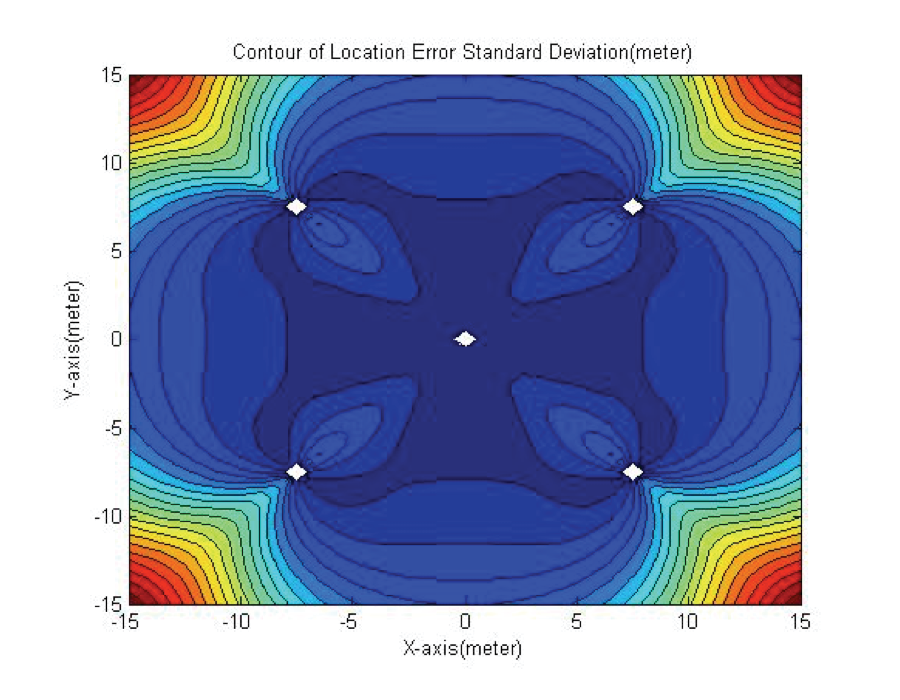
\includegraphics[]{pictures/5_7.eps}}
		\end{tabular}
	\end{center}
	\caption{Scenario II: Four iBeacons in the Middle and One at the Center.}
	\label{fig: 5.7}
\end{figure}



\begin{equation}
\sigma^2_1 = tr\{cov_\theta (\hat{x}_1, \hat{y}_1)\} = \textrm{var}_\theta (\hat{x}_1) +  \textrm{var}_\theta (\hat{y}_1) = tr(
I(\theta_1)^{-1})
\end{equation}

The derivation of 2D CRLB~\cite{pat}~\cite{qi} can be expanded into 3D cases by adding a z-axsis and apply the similar mathematics, meaning that $\theta_1 = [x_1, y_1]$ should be changed into $\theta_1 = [x_1, y_1, z_1]$. Accordingly, the equation (4.6) should be re-written as 

\begin{equation}
I_{\theta_1, \theta_i} = -E\nabla_{\theta_1, \theta_i}(\nabla_{\theta_1, \theta_i} \ln l (X|\theta_1,\theta_i)) = 
\begin{bmatrix}
I_{xx} & I_{xy} & I_{xz} \\
I_{xy} & I_{yy} & I_{yz} \\
I_{xz} & I_{yz} & I_{zz}
\end{bmatrix}
(\textrm{3D situation})
\end{equation}

The calculation of $I_{zz}$ is similar to that of $I_{xz}$ and $I_{yz}$, so that the CRLB in 3D situation comes to

%%%%%% figure is for next section
\begin{figure}[htb]
	\begin{center}
		\begin{tabular}{c}
			\scalebox{0.9}{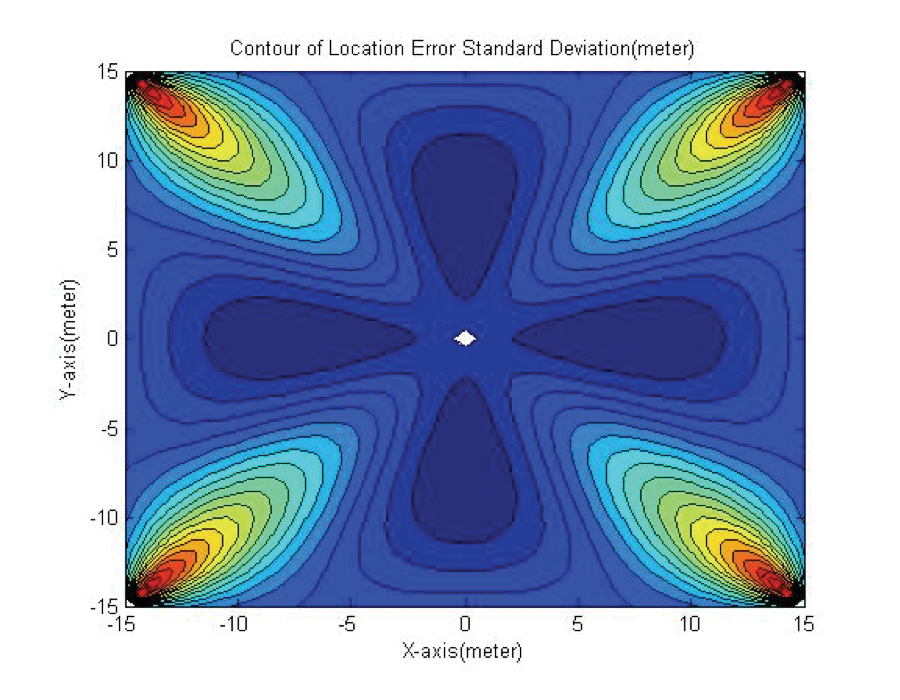
\includegraphics[]{pictures/5_6.eps}}
		\end{tabular}
	\end{center}
	\caption{Scenario I: Four iBeacons at the Corners and One at the Center.}
	\label{fig: 5.6}
\end{figure}


\begin{equation}
\sigma^2_1 = tr\{cov_\theta (\hat{x}_1, \hat{y}_1, \hat{z}_1)\} = \textrm{var}_\theta (\hat{x}_1) +  \textrm{var}_\theta (\hat{y}_1) + \textrm{var}_\theta (\hat{z}_1)= tr(
I(\theta_1)^{-1})
\end{equation}

In this section, we use CRLB as an evaluation metric for the performance of iBeacon based in-room localization system.

%%%%%%%%%%%%%%%%%%%%%%%%%%%%%%%%%%%%%%%%%%%%%%%%%%%%%%%%%%%%%%%%%%%%%%%%%%%%%%%%%%%%%%%%%%%%%%%%%%%%%%%%%%%%%%%%%%%%%%%


\subsection{Performance Evaluation Regarding Deployment Patterns.}
As we discussed before, there are 3 scenarios we analyze and compare inorder to evaluate the feasibility and effectiveness. From the Matlab we have such conclusions. The simulation conditions for location error analysis are as follows:

\begin{figure}[htb]
	\begin{center}
		\begin{tabular}{c}
			\scalebox{0.9}{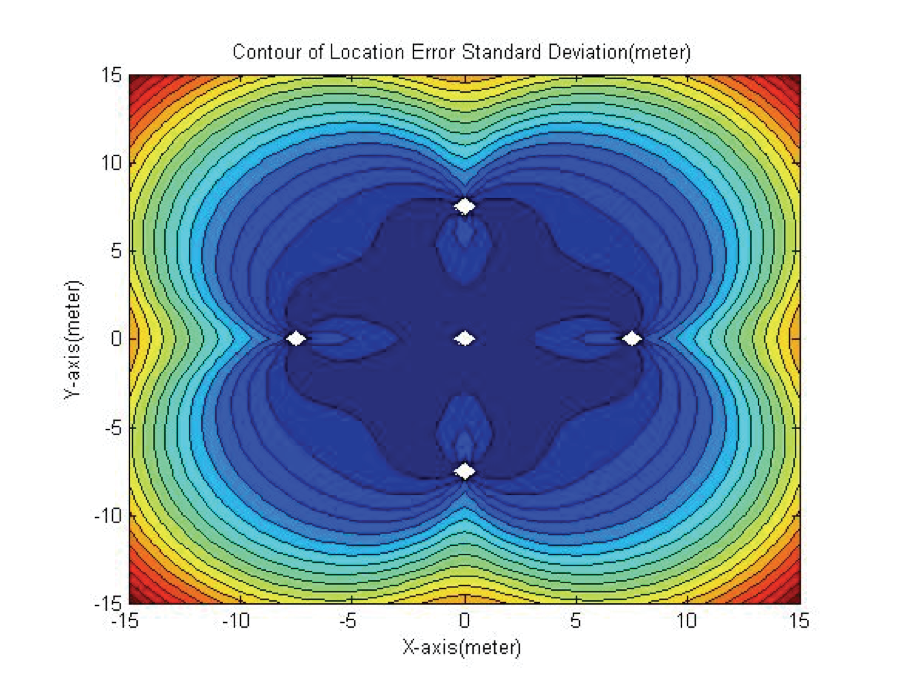
\includegraphics[]{pictures/5_8.eps}}
		\end{tabular}
	\end{center}
	\caption{Scenario III: Four iBeacons in the Middle with rotation and One at the Center.}
	\label{fig: 5.8}
\end{figure}

Pr(0) = 160W = 52dBm, and  α = 2.4583 which is the mean of the  α  values of real path-loss model derived in part II (shown in Table-1).

In the first scenario, we assume that there are five APs installed in a building with their coordinates being AP 1 (15m, 15m), AP 2 (15m, -15m), AP 3 (-15m, -15m), AP 4 (-15m, 15m), and AP 5 (0.1m, 0.1m). If an MS at a given location receives signals from these APs, its position can be determined by triangulation or least square estimation. The simulation result is shown in Fig~\ref{fig: 5.6}.

\begin{figure}[htb]
	\begin{center}
		\begin{tabular}{c}
			\scalebox{0.9}{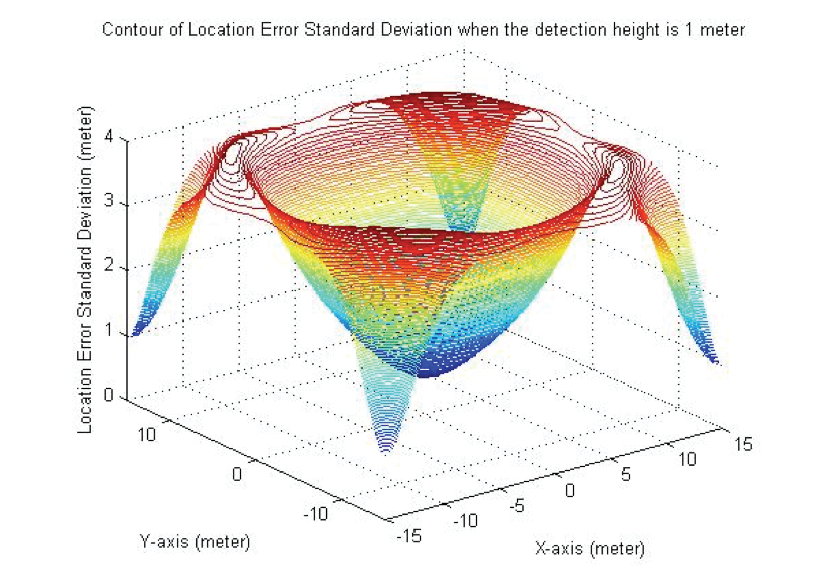
\includegraphics[]{pictures/5_9.eps}}
		\end{tabular}
	\end{center}
	\caption{Contour of Estimate Location Error in 3D When the Detection Height is One Meter.}
	\label{fig: 5.9}
\end{figure}


Then we move the four iBeacons from four corners to the middle area of the room to reach the second scenario shown in Fig~\ref{fig: 5.7} and also make such type figure. When we come to the last scenario shown in Fig~\ref{fig: 5.8}, we just do a rotation of 90 degrees with the four iBeacons in the middle and reach the result. 

Since the nursery room is a cube in reality, we extend the formula and simulation conditions from 2D to 3D. Z axis is introduced into the original x × y plane and we also move the fifth iBeacon from the middle of ground up to the middle of the roof. Due to plotting of a 4D figure is impossible, we give the figure in a particular height. Fig~\ref{fig: 5.9} shows the contour of estimate location error in 3D with one-meter detection height.


\section{Results and Discussion}
In this section, we compare the CDF of the error in three different deployment patterns to present the results of our in-room deployments. Later on, we also observe the influence of number of iBeacon by simulations in the same conditions to show the most efficient deployment method.

\begin{figure}[htb]
	\begin{center}
		\begin{tabular}{c}
			\scalebox{0.9}{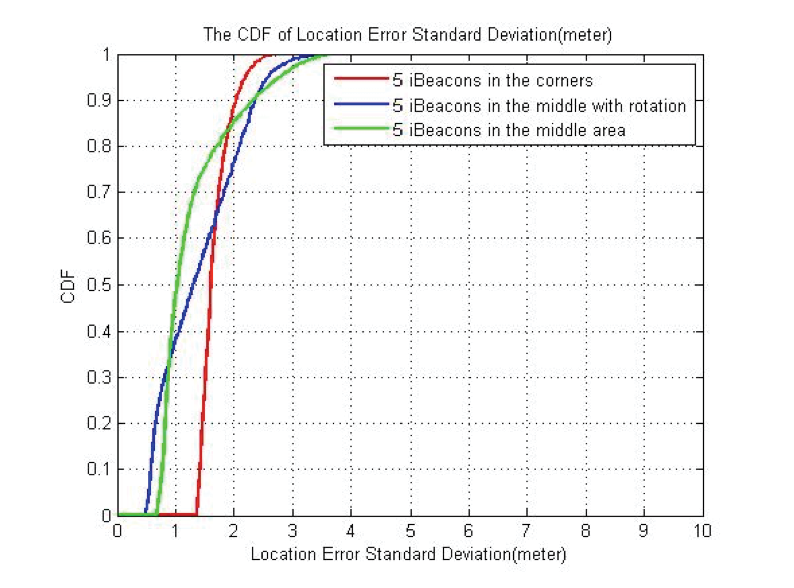
\includegraphics[]{pictures/4_10.eps}}
		\end{tabular}
	\end{center}
	\caption{CDF Comparison for Different Deployments.}
	\label{fig: 5.10}
\end{figure}

\begin{figure}[htb]
	\begin{center}
		\begin{tabular}{c}
			\scalebox{0.9}{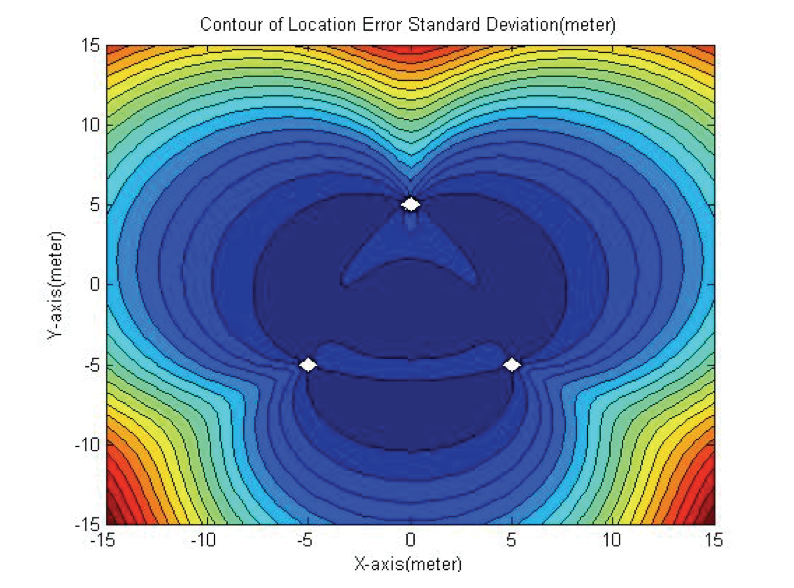
\includegraphics[]{pictures/4_11.eps}}
		\end{tabular}
	\end{center}
	\caption{Contour of estimate location error of 3 iBeacons.}
	\label{fig: 5.11}
\end{figure}

\begin{figure}[htb]
	\begin{center}
		\begin{tabular}{c}
			\scalebox{0.9}{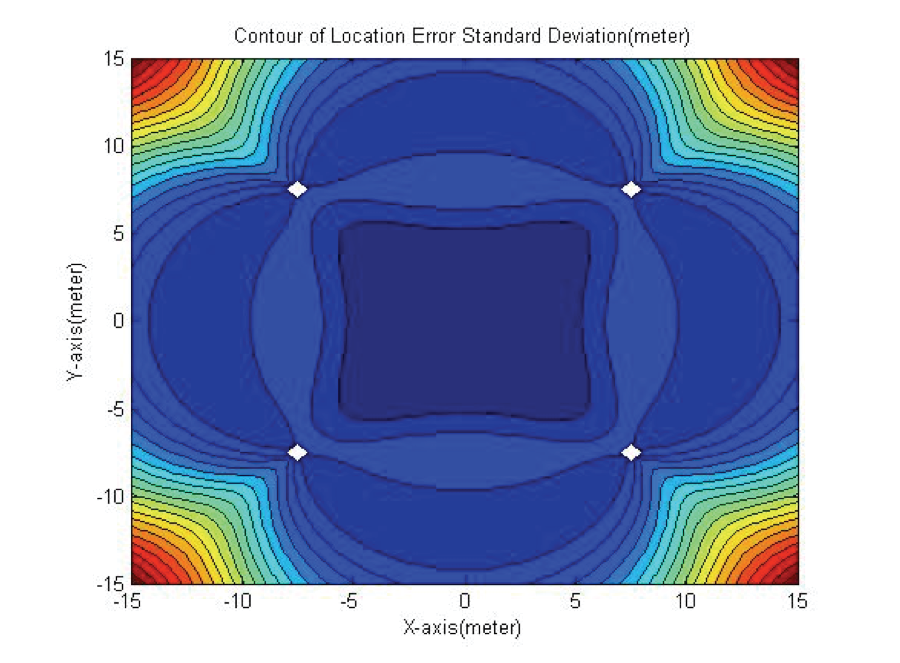
\includegraphics[]{pictures/4_12.eps}}
		\end{tabular}
	\end{center}
	\caption{Contour of estimate location error of 4 iBeacons.}
	\label{fig: 5.12}
\end{figure}

\begin{figure}[htb]
	\begin{center}
		\begin{tabular}{c}
			\scalebox{0.9}{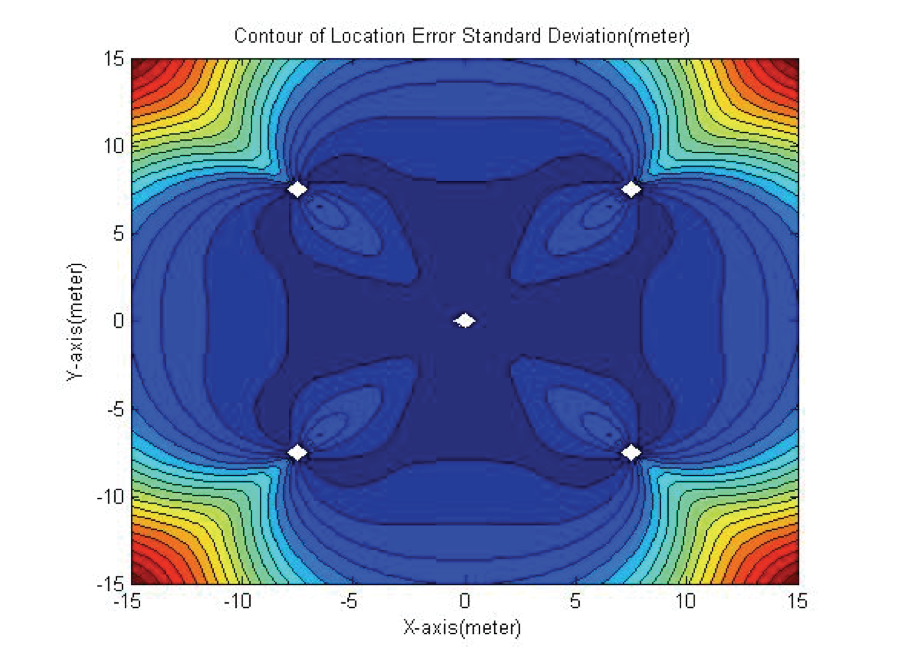
\includegraphics[]{pictures/4_13.eps}}
		\end{tabular}
	\end{center}
	\caption{Contour of estimate location error of 5 iBeacons.}
	\label{fig: 5.13}
\end{figure}

\subsection{Effect of Different Deployment Patterns.}
In order to observe the performance of 3 different scenarios directly, we calculate the CDF of estimation of location error and compare them. In Fig~\ref{fig: 5.10}. we can see that the deployment with four iBeacons in the middle area has the best performance, this is probably because in this scenario it owes the highest overlap rate of coverage area, which means that most part of the room can be located by 2 or more iBeacons and results in the highest accuracy.

Apart from that, based on the figures we give before, we also calculate the means and variances of CDF of the location estimation error in the different scenarios. From Fig~\ref{fig: 5.10} we can claim that 5 iBeacons in the middle area performs best (green line in Fig~\ref{fig: 5.10}). The comparison is in table-3.

\subsection{Effect of Different Number of iBeacons}
Apart from the different deployment patterns, it is more reasonable to take into account the number of iBeacon. With the same simulation conditions in Matlab, we conclude the performance with 3, 4 and 5 iBeacons in the same environment. One of the simulations can be viewed in Fig~\ref{fig: 5.11}.

Above is the error estimation result with 3,4 and 5 iBeacons in the middle area since we have already certified that the deployment in the middle owes the best performance. In addition, we can still calculate the CDF of the location estimation error to compare them and reach a conclusion. 

\begin{figure}[htb]
	\begin{center}
		\begin{tabular}{c}
			\scalebox{0.9}{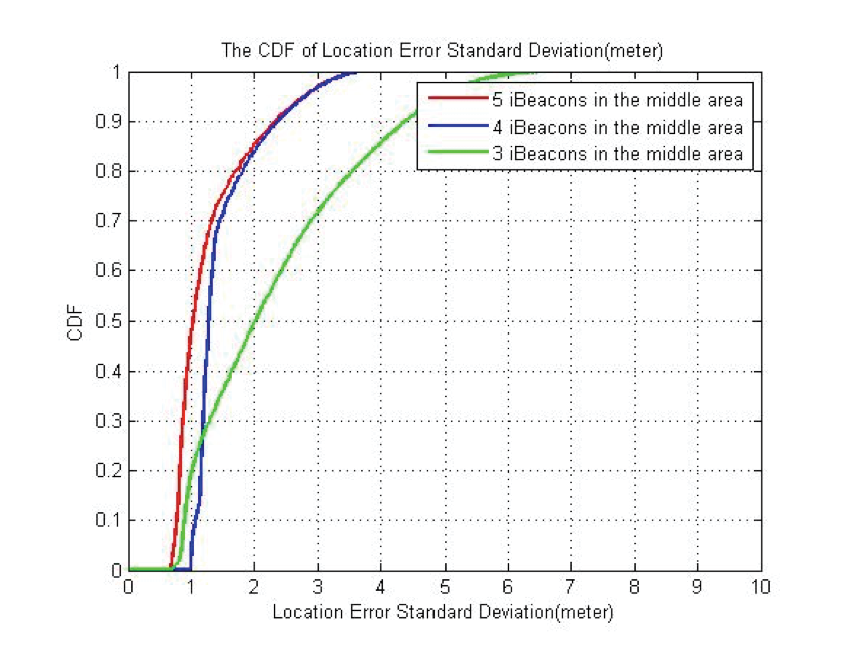
\includegraphics[]{pictures/4_14.eps}}
		\end{tabular}
	\end{center}
	\caption{CDF comparison for different number of iBeacons.}
	\label{fig: 5.14}
\end{figure}

Obviously, 5 iBeacons owes the best performance, however, we can find that the improvement from 3 iBeacons to 4 iBeacons is significant while the improvement from 4 iBeacons to 5 iBeacons is negligible. So we can assert that the deployment with 4 iBeacons in the middle area contains the highest efficiency. The overall performance is concluded in table-4.

\chapter{Conclusion and Future Work}
In this master thesis, we first developed the iBeacon based intelligent in-room presence detection system and evaluated its performance. In order to extract the RSSI data of iBeacon to do further analysis, we developed our own iOS application based on the Software Development Kit provided by Estimote. We defined three scenarios of human movement, which are entering, leaving, and passing the room. Based on the data we collected, we designed two algorithms to distinguish those three scenarios. To make sure that the place we put the receiver won't affect the detection rate, we put the receiver in hand, pants pocket, and shirt pocket when we did performance evaluation of two algorithms. The detection rates of two algorithms are almost 100\%. We got the conclusion that both of the algorithms are reliable. Since single iBeacon approach required less iBeacons and the algorithm is simpler, we thought single iBeacon approach is adequate.  

After that, we built the path-loss model of iBeacon and did the performance evaluation of iBeacon based in-room localization. We calculated the Estimote iBeacon model and computed real path-loss model. After comparing CDF of two models we found out the real path-loss model is better. We evaluated the performance of different deployment patterns of iBeacon by using CRLB. When there were five iBeacons in the room, putting one at the center of the room and four at the midpoints of diagonals will reach the best performance. We also studied the optimal number of iBeacon which can provide the best performance. The conclusion is we can improve the performance by using more iBeacon, but the improvement is negligible when the number of iBeacons is larger than five.

Even though the iBeacon based system has been deeply investigated in this thesis, the system still has various potential advantages underexplore. As for the future work, we plan to include the inertial sensors inside the smart receivers into our in-room localization solution. In this way, the original RF based localization can be promoted to a hybrid localization and therefore, increase the in-room localization accuracy.



% Let's assume this is the end of your thesis text.

% Now come appendices, if you had any.
% Appendices are automatically numbered, just like everything else in
% LaTeX. But only after you gave this command
\appendix

\chapter{More to say}

\section{A section within an appendix.}
This is an appendix.


% Last and least (at least, that's what the library says) - the
% Bibliography.


% you can save some space by having the bibliography singlespaced, if you want
\singlespacing

%
% You should become familiar with the BibTeX program, which
% uses a *.bib-file to collect all citations that you have. It's a lot
% prettier than typing all the citations right into the document. The 
% reference to citations also works well that way, but the exact 
% explanation of that will be on the CS-GSO homepage, whenever I'll ever 
% have time for that.
%
%
% If you use BibTeX, the bibliography is very easy. You refer to
% citations in the text with \cite{tag}, where tag is the tag that you
% defined in the bib-file.
% Then, you run bibtex once in a while during compilation, and the
% rest is done in two lines:


\bibliographystyle{alpha}
\bibliography{foo}

% which assumes a file foo.bib in your working directory.
% The word ``Bibliography'' will appear in your document as soon as
% you used ``bibtex'' on the command line.
%
% For reference on this, refer to the CS-GSO homepage.

%============================
%That's all, folks. Have fun.
%
%                     Andreas
%============================


\end{document}









